\documentclass[a5paper, 11pt]{extarticle}
\usepackage[utf8]{inputenc}
\usepackage[T1]{fontenc}
\usepackage{graphicx}
\usepackage{longtable}
\usepackage{tabularray}
\usepackage{wrapfig}
\usepackage{rotating}
\usepackage{float}
\usepackage[normalem]{ulem}
\usepackage{amsmath}
\usepackage{amssymb}
\usepackage{capt-of}
\usepackage{hyperref}
\usepackage{fontspec}
\usepackage[russian]{babel}
\usepackage{indentfirst}
\usepackage{relsize}
\usepackage{multicol}
\usepackage{MnSymbol}
\usepackage[
    left=10mm,
    right=10mm,
    top=15mm,
    bottom=15mm
]{geometry}
\usepackage{amsthm}
\usepackage{enumitem}
\usepackage{unicode-math}
\usepackage[math]{cellspace}
\usepackage{mathtools}
\usepackage{caption}
\usepackage{array}

\setmainfont{PT Astra Serif}
\setmathfont{Latin Modern Math}
\setmathfont[range=\setminus]{Asana Math}
\setmathfont[range=\varnothing]{Asana Math}

\captionsetup{width=\textwidth}

\newcommand{\PreserveBackslash}[1]{\let\temp=\\#1\let\\=\temp}
\newcolumntype{C}[1]{>{\PreserveBackslash\centering}p{#1}}
\newcolumntype{R}[1]{>{\PreserveBackslash\raggedleft}p{#1}}
\newcolumntype{L}[1]{>{\PreserveBackslash\raggedright}p{#1}}

\pagestyle{plain}

\theoremstyle{definition}
\newtheorem{theorem}{Теорема}[subsection]
\renewcommand{\thetheorem}{\arabic{theorem}}

\newtheorem*{theorem*}{Теорема}

\newtheorem{lemma}{Лемма}[subsection]
\renewcommand{\thelemma}{\arabic{lemma}}

\newtheorem{property}{Свойство}[subsection]
\renewcommand{\theproperty}{\arabic{property}}

\newtheorem{example}{Пример}[subsection]
\renewcommand{\theexample}{\arabic{example}}

\newtheorem*{example*}{Пример}

\theoremstyle{definition}
\newtheorem{definition}{Определение}[subsection]
\renewcommand{\thedefinition}{\arabic{definition}}

\theoremstyle{definition}
\newtheorem*{definition*}{Определение}

\newtheorem{consequence}{Следствие}[subsection]
\makeatletter
\counterwithin{consequence}{property}
\counterwithin{consequence}{theorem}
\makeatother
\renewcommand{\theconsequence}{\arabic{consequence}}

\newtheorem*{consequence*}{Следствие}

\newtheorem{note}{Замечание}[subsection]
\makeatletter
\counterwithin{note}{property}
\counterwithin{note}{theorem}
\makeatother
\renewcommand{\thenote}{\arabic{note}}

\newtheorem*{note*}{Замечание}

\numberwithin{figure}{section}
\numberwithin{table}{section}

\newcommand{\intersects}{\mathord{\bigcirc\kern-0.5em{\bigcirc}}}
\newcommand{\symdiff}{\medtriangleup}

\newcommand*{\divby}{\mathrel{\rotatebox{90}{$\hskip-1pt.{}.{}.$}}}%

\newcommand{\newpar}{$ $\par\nobreak\ignorespaces}
\renewenvironment{proof}{{\noindent\bfseries Доказательство.}}{\smallskip\newpar \hfill\textit{Что и требовалось доказать.}}
\usepackage[x11names]{xcolor}
\author{Daniil Shvalov}
\date{\today}
\title{}
\hypersetup{
    pdfauthor={Daniil Shvalov},
    pdftitle={},
    pdfkeywords={},
    pdfsubject={},
    pdflang={Russian}}

% Define math operators
\DeclareMathOperator{\rang}{rang}
\DeclareMathOperator{\Ima}{Im}
\DeclareMathOperator{\defect}{def}
\renewcommand*{\nok}{\text{НОК}}
\DeclareMathOperator{\biglor}{\mathrel{\raisebox{-.4ex}{$\mathlarger{\mathlarger{\mathlarger{\mathlarger{\lor}}}}$}}}
\DeclareMathOperator{\bigland}{\mathrel{\raisebox{-.4ex}{$\mathlarger{\mathlarger{\mathlarger{\mathlarger{\land}}}}$}}}


% Draw line in matrix
\makeatletter
\renewcommand*\env@matrix[1][*\c@MaxMatrixCols c]{%
    \hskip -\arraycolsep
    \let\@ifnextchar\new@ifnextchar
    \array{#1}}
\makeatother

\setlist[itemize]{itemsep=0.5em,topsep=0em,parsep=0em}
\setlist[enumerate]{itemsep=0.5em,topsep=0em,parsep=0em}

\makeatletter
\def\thm@space@setup{\thm@preskip=1pt
    \thm@postskip=1pt}
\makeatother

\def\lets{%
    \mathord{\setbox0=\hbox{$\exists$}%
        \hbox{\kern 0.125\wd0%
            \vbox to \ht0{%
                \hrule width 0.75\wd0%
                \vfill%
                \hrule width 0.75\wd0}%
            \vrule height \ht0%
            \kern 0.125\wd0}%
    }%
}

\begin{document}

\hypersetup{linktoc = all, colorlinks = true, urlcolor = DodgerBlue4, citecolor = PaleGreen1, linkcolor = black}
\tableofcontents
\hypersetup{linktoc = all, colorlinks = true, urlcolor = DodgerBlue4, citecolor = PaleGreen1, linkcolor = blue}
\newpage

\section{Множества и отношения}

\subsection{Основные понятия}

\textbf{Множество} -- любая определенная совокупность объектов. Элементы множества различны и отличными друг от друга.

Под \textbf{множеством} понимают любой набор определенных и различимых между собой объектов, мыслимый как единое целое. Объекты, из которых составлено множество, называются его \textbf{элементами}.

Множества обычно обозначатся заглавными латинскими буквами: \(A, B, C, \ldots\). Элементы множества обозначаются строчными латинскими буквами: \(a, b, c, \ldots\).

Для обозначения того, что объект \(x\) является, либо не является элементом множества \(A\), используют символику:
\begin{itemize}
    \item \(x \in A\) -- объект \(x\) является элементом множества \(A\).
    \item \(x \notin A\) -- объект \(x\) не является элементом множества \(A\).
\end{itemize}

Множество, не содержащее ни одного элемента, называется \textbf{пустым} и обозначается символом \(\varnothing\).

Множество, из элементов которого составляют конкретное множество, называют \textbf{универсальным} и обозначают символом \(U\).

Множество \(U\) называется \textbf{универсальным} для данной задачи, если все рассматриваемые в этой задаче множества являются его подмножествами.

Множества можно изображать с помощью кругов, которые называются \textbf{кругами Эйлера} или \textbf{диаграммами Венна}. Универсальное множество принято обозначать прямоугольником.

Способы задания множества:
\begin{enumerate}
    \item перечислением всех элементов множества (в фигурных скобках через запятую):
          \[
              A = \{1, 2, 3, 4\};
          \]
    \item характеристическим предикатом, который описывает свойство всех элементов, входящих в множество. Характеристический предикат записывается после двоеточия или символа <<\(\mid\)>>:
          \[
              A = \{x: P(x)\}
              \quad
              \lor
              \quad
              A = \{x \mid P(x)\}
          \]
          где \(P(x)\) -- характеристический предикат.
\end{enumerate}

Обозначения числовых множеств:
\begin{itemize}
    \item \(\mathbb{N}\) -- множества натуральных чисел, \(\mathbb{N} = \{1, 2, 3, \ldots\}\);
    \item \(\mathbb{Z}\) -- множества целых чисел, \(\mathbb{Z} = \{\ldots, -2, -1, 0, 1, 2, \ldots\}\);
    \item \(\mathbb{Q}\) -- множество рациональных числе, \(\mathbb{Q} = \Big\{\dfrac{m}{n} (m \in \mathbb{Z}, n \in \mathbb{N})\Big\}\);
    \item \(\mathbb{R}\) -- множество действительных (вещественных) чисел;
    \item \(\mathbb{C}\) -- множество комплексных чисел.
\end{itemize}

\subsection{Сравнение множеств}

Множество \(A\) называется \textbf{подмножеством} множества \(B\) (множество \(A\) содержится в \(B\), множество \(B\) включает множество \(A\)), если каждый элемент множества \(A\) является элементом множества \(B\):
\[
    A \subseteq B
    \iff
    \forall x \in A \implies x \in B.
\]
\(B\) называется \textbf{надмножеством} множества \(A\).

Под определению пустое множество является подмножеством всех множеств:
\[
    \forall M \implies \varnothing \subseteq M.
\]
Универсальное множество содержит все множества:
\[
    \forall M \implies M \subseteq U.
\]

Два множества называют \textbf{равными}, если они являются подмножествами друг друга:
\[
    A = B
    \iff
    A \subseteq B \land B \subseteq A.
\]

Если \(A \subseteq B\) и \(A \neq B\), то множество \(A\) называется \textbf{собственным} подмножеством множества \(B\), а \(B\) -- \textbf{собственным} надмножеством \(A\).

Множества \(A\) и \(B\) \textbf{сравнимые}, если \(A \subseteq B \lor B \subseteq A\). Иначе множества называются \textbf{несравнимыми}.

\subsection{Свойства включения множеств}

\begin{property}
    \[
        \forall A \implies A \subseteq A.
    \]
\end{property}

\begin{property}
    \[
        \forall A, B : A \subseteq B \land B \subseteq A \implies A = B.
    \]
\end{property}

\begin{property}
    \[
        \forall A, B, C : A \subseteq B \land B \subseteq C \implies A \subseteq C.
    \]
\end{property}

\subsection{Мощность множества}

Говорят, что между множествами \(A\) и \(B\) установлено \textbf{взаимно-однозначное соответствие}, если каждому элементу множества \(A\) поставлен в соответствие один и только один элемент множества \(B\), и каждому элементу множества \(B\) поставлен в соответствие один и только один элемент множества \(A\):
\[
    A \sim B
    \iff
    \begin{dcases}
        \forall a \in A \mapsto !b \in B \\
        \forall b \in B \mapsto !a \in A
    \end{dcases}
\]

Два множества (конечных или бесконечных) имеют \textbf{одинаковую мощность}, если между этими множествами можно установить взаимно-однозначное соответствие. В этом случае говорят, что множества \(A\) и \(B\) \textbf{изоморфны}, имеют одинаковую \textbf{мощность}, или что они \textbf{равномощны}, и обозначают \(|A| = |B|\).

Множество \(A\) называется \textbf{конечным}, если у него нет равномощного собственного подмножества:
\[
    \forall B: B \subseteq A \land |B| = |A| \implies B = A.
\]
Для конечного множества используется запись \(|A| < \infty\).

Множество \textbf{бесконечно} тогда и только тогда, когда оно имеет одинаковую мощность с некоторым своим подмножеством, не совпадающим с самим этим множеством:
\[
    \exists B: B \subseteq A \land |B| = |A| \land B \neq A.
\]
То есть бесконечное множество равномощно некоторому своему собственному подмножеству. Для бесконечного множества используется запись \(|A| = \infty\).

Множество \(X\) называется \textbf{счетным}, если его мощность равна мощности множества натуральных чисел, т. е. \(|X| = |\mathbb{N}|\).

Говорят, что множество \(X\) -- множество \textbf{мощности континуума}, если его мощность равна мощности множества точек на отрезке \([0, 1]\).

\begin{theorem*}[Теорема Кантора о несчетности]
    Отрезок \([0, 1]\) несчетен, т. е.
    \[
        |[0, 1]| > |\mathbb{N}|.
    \]
\end{theorem*}

\subsection{Операции над множествами}

\textbf{Объединением} двух множеств называется множество, содержащее все элементы обоих множеств:
\[
    A \cup B = \{x \mid x \in A \lor x \in B\}.
\]

\begin{figure}[H]
    \centering
    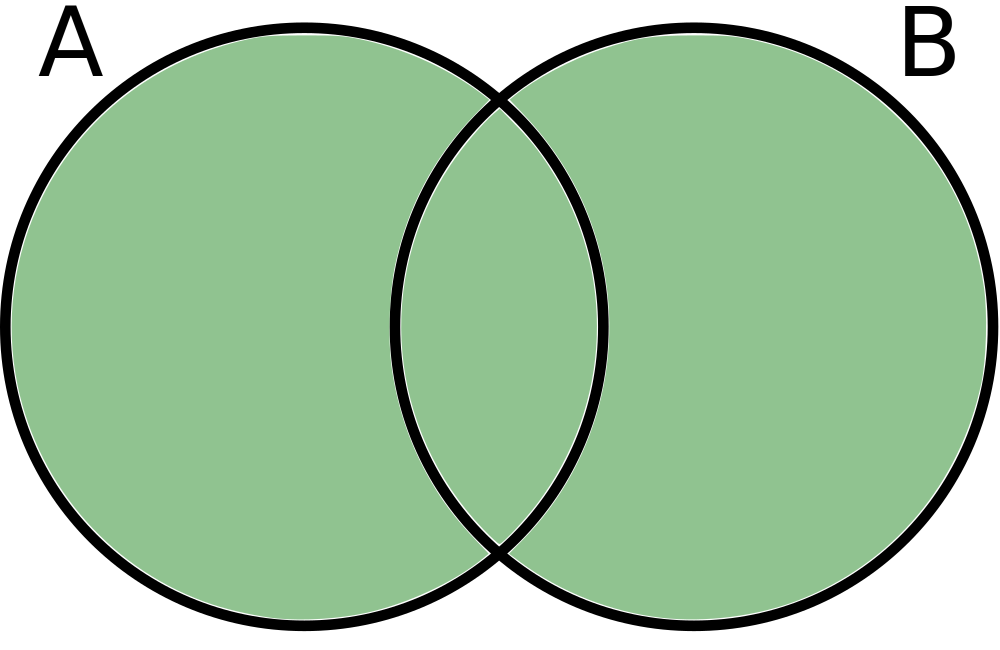
\includegraphics[width=0.5\textwidth]{images/set-combining.png}
    \caption{Объединение двух множеств}
\end{figure}

\textbf{Пересечением} двух множеств называется множество, состоящее из элементов, входящих в каждое из множеств \(A\) и \(B\):
\[
    A \cap B = \{x \mid x \in A \land x \in B\}.
\]

\begin{figure}[H]
    \centering
    
\includegraphics[width=0.5\textwidth]{images/set-intersection.png}
    \caption{Пересечение двух множеств}
\end{figure}

\textbf{Разностью} множеств \(A\) и \(B\) называется множество, состоящее из всех элементов множества \(A\), не содержащихся в множестве \(B\):
\[
    A \setminus B = \{x \mid x \in A \land x \notin B\}.
\]

\begin{figure}[H]
    \centering
    
\includegraphics[width=0.5\textwidth]{images/set-difference.png}
    \caption{Разность двух множеств}
\end{figure}

\textbf{Симметрической разностью} множеств \(A\) и \(B\) называется множество, состоящее из всех элементов множества \(A\), не содержащихся в множестве \(B\), и всех элементов множества \(B\), не содержащихся в множестве \(A\):
\[
    A \symdiff B = \{x \mid (x \in A \land x \notin B) \lor (x \notin A \land x \in B)\}.
\]

\begin{figure}[H]
    \centering
    
\includegraphics[width=0.5\textwidth]{images/set-sym-difference.png}
    \caption{Симметрическая разность двух множеств}
\end{figure}

\textbf{Дополнением} (дополнением до универсального множества \(U\)) множества \(A\) называется множество, состоящее из всех элементов универсального множества, не содержащихся в множестве \(A\):
\[
    \bar{A} = \{x \mid x \notin A\}.
\]

\begin{figure}[H]
    \centering
    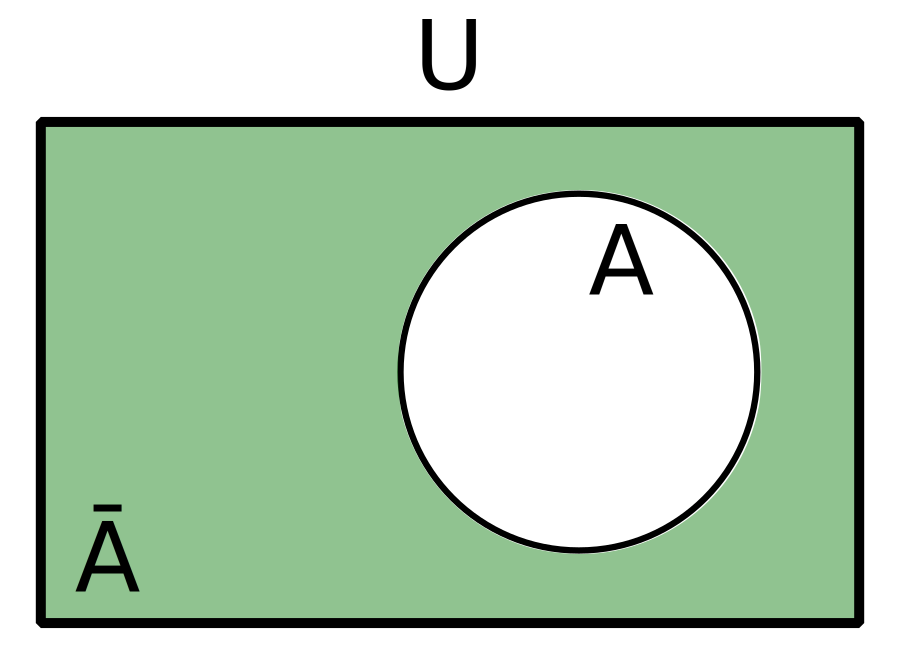
\includegraphics[width=0.55\textwidth]{images/set-complement.png}
    \caption{Дополнение множества}
\end{figure}

\subsection{Свойства операций над множествами}

\begin{property}[Идемпотентность]
    \[
        A \cup A = A,
        \quad
        A \cap A = A.
    \]
\end{property}

\begin{property}[Коммутативность]
    \[
        A \cup B = B \cup A,
        \quad
        A \cap B = B \cap A.
    \]
\end{property}

\begin{property}[Ассоциативность]
    \[
        A \cup (B \cup C) = (A \cup B) \cup C,
        \quad
        A \cap (B \cap C) = (A \cap B) \cap C.
    \]
\end{property}

\begin{property}[Дистрибутивность]
    \[
        A \cup (B \cap C) = (A \cup B) \cap (A \cup C),
        \quad
        A \cap (B \cup C) = (A \cap B) \cup (A \cap C).
    \]
\end{property}

\begin{property}[Поглощение]
    \[
        (A \cap B) \cup A = A,
        \quad
        (A \cup B) \cap A = A.
    \]
\end{property}

\begin{property}[Свойства нуля]
    \[
        A \cup \varnothing = A,
        \quad
        A \cap \varnothing = \varnothing.
    \]
\end{property}

\begin{property}[Свойства единицы]
    \[
        A \cup U = U,
        \quad
        A \cap U = A.
    \]
\end{property}

\begin{property}[Инволютивность]
    \[
        \bar{\bar{A}} = A.
    \]
\end{property}

\begin{property}[Законы де Моргана]
    \[
        \overline{A \cap B} = \bar{A} \cup \bar{B},
        \quad
        \overline{A \cup B} = \bar{A} \cap \bar{B}.
    \]
\end{property}

\begin{property}[Свойства дополнения]
    \[
        A \cup \bar{A} = U,
        \quad
        A \cap \bar{A} = \emptyset.
    \]
\end{property}

\begin{property}[Свойство разности]
    \[
        A \setminus B = A \cap \bar{B}.
    \]
\end{property}

\begin{property}[Свойство симметрической разности]
    \[
        A \symdiff B = (A \setminus B) \cap (B \setminus A).
    \]
\end{property}

\subsection{Обобщенные тождества алгебры множеств}

\begin{property}[Обобщенная дистрибутивность]
    \[
        A \cap \bigcup_{i = 1}^n B_i = \bigcup_{i = 1}^n (A \cap B_i);
        \qquad
        A \cup \bigcap_{i = 1}^n B_i = \bigcap_{i = 1}^n (A \cup B_i).
    \]
\end{property}

\begin{property}[Обобщенный закон де Моргана]
    \[
        \overline{\bigcup_{i = 1}^n A_i} = \bigcap_{i = 1}^n \overline{A_i};
        \qquad
        \overline{\bigcap_{i = 1}^n A_i} = \bigcup_{i = 1}^n \overline{A_i}.
    \]
\end{property}

\subsection{Булеан}

Множество всех подмножеств \(A\) называется \textbf{булеаном} множества \(A\) и обозначается \(2^A\):
\[
    2^A = \{B \mid B \subseteq A\}.
\]

\begin{theorem*}
    Если множество \(A\) конечно, то \(|2^A| = 2^{|A|}\).
\end{theorem*}

\subsection{Методы доказательств теоретико-множественных тождеств}

\subsubsection{Метод двух включений}

Пусть левая часть теоретико-множественного тождества определяет множество \(X\), а правая часть -- множество \(Y\). Чтобы доказать равенство множеств \(X\) и \(Y\), достаточно доказать два включения \(X \subseteq Y\) и \(Y \subseteq X\), т. е. доказать, что
\[
    \forall x \in X \implies x \in Y
    \quad \land \quad
    \forall x \in Y \implies x \in X.
\]

Докажем этим методом тождество
\[
    A \symdiff B = (A \cup B) \setminus (A \cap B).
\]

Пусть \(x \in A \symdiff B\). Тогда, согласно определению симметрической разности
\begin{gather*}
    x \in (A \symdiff B) \implies
    x \in ((A \setminus B) \cup (B \setminus A)) \implies \\ \implies
    (x \in A \land x \notin B) \lor (x \in B \land x \notin A) \implies \\ \implies
    (x \in (A \cup B) \land x \notin (A \cap B)) \lor (x \in (A \cup B) \land x \notin (A \cap B)) \implies \\ \implies
    x \in (A \cup B) \land x \notin (A \cap B) \implies
    x \in ((A \cup B) \setminus (A \cap B)).
\end{gather*}

Таким образом доказано, что \(A \symdiff B \subseteq (A \cup B) \setminus (A \cap B)\). Докажем обратное включение \((A \cup B) \setminus (A \cap B) \subseteq A \symdiff B\):
\begin{gather*}
    x \in ((A \cup B) \setminus (A \cap B)) \implies
    x \in (A \cup B) \land x \notin (A \cap B) \implies \\ \implies
    (x \in A \land x \notin B) \lor (x \in B \land x \notin A) \implies \\ \implies
    x \in ((A \setminus B) \cup (B \setminus A)) \implies
    x \in (A \symdiff B).
\end{gather*}

Оба включения имеют место и тождество доказано.

\subsubsection{Метод эквивалентных преобразований}

Теоретико-множественные тождества можно доказывать, используя свойства операций над множествами. Для этого нужно преобразовать левую часть в правую, или правую -- в левую, или правую и левую часть в некоторое третье выражение.

Докажем этим методом тождество:
\[
    (A \cap B) \symdiff (A \cap C) = A \cap (B \symdiff C).
\]

Преобразуем левую часть к правой:
\begin{gather*}
    (A \cap B) \symdiff (A \cap C) = \\ =
    ((A \cap B) \cup (A \cap C)) \cap \overline{(A \cap B) \cap (A \cap C)} = \\ =
    (A \cap (B \cup C)) \cap (\overline{A \cap B} \cup \overline{A \cap C}) = \\ =
    (A \cap (B \cup C)) \cap (\bar{A} \cup \bar{B} \cup \bar{A} \cup \bar{C}) = \\ =
    (A \cap (B \cup C)) \cap (\bar{A} \cup \bar{B} \cup \bar{C}) = \\ =
    ((A \cap (B \cup C)) \cap \bar{A}) \cup ((A \cap (B \cup C)) \cap (\bar{B} \cup \bar{C})) = \\ =
    (B \cup C) \cap (A \cap (\bar{B} \cup \bar{C})) = \\ =
    (A \cap (B \cup C)) \cap (A \cap (\overline{B \cap C})) = \\ =
    A \cap ((B \cup C) \cap (\overline{B \cap C})) = \\ =
    A \cap (B \symdiff C).
\end{gather*}

\subsubsection{Метод характеристических функций}

Характеристическая функция \(\chi_A\) множества \(A\) для \(x \in U\) определяется следующим образом:
\[
    \begin{dcases}
        \chi_A(x) = 1, \quad x \in A \\
        \chi_A(x) = 0, \quad x \notin A
    \end{dcases}
\]
Для характеристической функции справедливы следующие тождества:
\begin{enumerate}
    \item \(\chi_A^2(x) = \chi_A(x)\);
    \item \(\chi_{A \cap B}(x) = \chi_A(x) \cdot \chi_B(x)\);
    \item \(\chi_{A \cup B}(x) = \chi_A(x) + \chi_B(x) - \chi_A(x) \cdot \chi_B(x)\);
    \item \(\chi_{\bar{A}} = 1 - \chi_A(x)\);
    \item \(\chi_{A \setminus B}(x) = \chi_A(x) - \chi_A(x) \cdot \chi_B(x)\);
    \item \(\chi_{A \symdiff B} = \chi_A(x) + \chi_B(x) - 2 \cdot \chi_A(x) \cdot \chi_B(x)\).
\end{enumerate}

Докажем этим методом тождество
\[
    (A \symdiff B) \cap C = (A \cap C) \symdiff (B \cap C).
\]

С одной стороны,
\begin{gather*}
    \chi_{(A \symdiff B) \cap C}(x) =
    \chi_{(A \symdiff B)}(x) \chi_C(x) = \\ =
    \big(\chi_A(x) + \chi_B(x) - 2 \chi_A(x) \chi_B(x)\big) \chi_C(x) = \\ =
    \chi_A(x) \chi_C(x) + \chi_B(x) \chi_C(x) - 2 \chi_A(x) \chi_B(x) \chi_C(x).
\end{gather*}

С другой стороны,
\begin{gather*}
    \chi_{(A \cap C) \symdiff (B \cap C)}(x) =
    \chi_{(A \cap C)}(x) + \chi_{(B \cap C)}(x) - 2 \chi_{(A \cap C)}(x) \chi_{(B \cap C)}(x) = \\ =
    \chi_A(x) \chi_C(x) + \chi_B(x) \chi_C(x) - 2 \chi_A(x) \chi_C(x) \chi_B(x) \chi_C(x) = \\ =
    \chi_A(x) \chi_C(x) + \chi_B(x) \chi_C(x) - 2 \chi_A(x) \chi_B(x) \chi_C(x).
\end{gather*}

Так как \(\chi_{(A \symdiff B) \cap C}(x) = \chi_{(A \cap C) \symdiff (B \cap C)}(x)\), тождество доказано.

\subsection{Упорядоченные пары и наборы}

\((a, b)\) -- упорядоченная пара объектов \(a\) и \(b\).

Равенство упорядоченных пар определяется следующим образом:
\[
    (a, b) = (c, d) \iff a = c \land b = d.
\]

Вообще говоря, \((a, b) \neq (b, a)\).

\((a_1, a_2, \ldots, a_n)\) -- упорядоченный набор из \(n\) элементов (\(n\)-ка, кортеж или (конечная) последовательность).

\(|(a_1, a_2, \ldots, a_n)|\) -- длина набора, т. е. количество элементов в наборе.

\begin{theorem*}
    Два набора одной длины равны, если равны их соответствующие элементы
    \[
        \forall n (a_1, \ldots, a_n) = (b_1, \ldots, b_n) \iff a_1 = b_1 \land \ldots \land a_n = b_n.
    \]
\end{theorem*}

\subsection{Прямое произведение множеств}

Прямым (декартовым) произведением двух множеств \(A\) и \(B\) называется множество всех упорядоченных пар, в которых первый элемент принадлежит \(A\), а второй принадлежит \(B\):
\[
    A \times B = \{(a, b) \mid a \in A \land b \in B\}.
\]
\[
    A \times B \neq B \times A.
\]

\begin{theorem*}
    Для конечных множества \(A\) и \(B\)
    \[
        |A \times B| = |A| \cdot |B|.
    \]
\end{theorem*}

Понятие прямого произведения допускает обобщение. Прямое произведение множеств \(A_1, \ldots, A_n\) -- это множество наборов (кортежей):
\[
    A_1 \times \ldots \times A_n
    =
    \{(a_1, \ldots, a_n) \mid a_1 \in A_1 \land \ldots \land a_n \in A_n\}.
\]
Множества \(A_i\) необязательно различны.

Степенью множества \(A\) называется его \(n\)-кратное произведение самого на себя:
\[
    A^n = \underbrace{A \times \ldots \times A}_{n-\text{раз}};
    \qquad
    |A^n| = |A|^n.
\]

\subsection{Бинарные отношения}

Бинарным отношением между множествами \(A\) и \(B\) называется такая тройка \(\langle A, B, R \rangle\), где \(R\) -- подмножество прямого произведения \(A\) и \(B\):
\[
    R \subset A \times B,
\]
Эти множества именуют следующим образом:
\begin{itemize}
    \item \(R\) -- график отношения;
    \item \(A\) -- область отправления;
    \item \(B\) -- область прибытия.
\end{itemize}

Область определения отношения:
\[
    \text{Dom} R = \{a \in A \mid \exists b \in B : (a, b) \in R\}.
\]

Область значений:
\[
    \text{Im} R = \{b \in B \mid \exists a \in A : (a, b) \in R\}.
\]

Если \(A = B\) (т. е. \(R \subset A^2\)), то говорят, что \(R\) есть отношение на множестве \(A\).

Для бинарных отношений обычно используется \textbf{инфиксная} форма записи:
\[
    aRb \iff (a, b) \in R \subset A \times B.
\]

Инфиксная форма позволяет более кратко записывать некоторые формы утверждений относительно отношений:
\[
    aRbRc \iff (a, b) \in R \land (b, c) \in R
\]

Обратное отношение:
\[
    R^{-1} = \{(b, a) \mid (a, b) \in R\} \subset B \times A.
\]

Дополнение отношения:
\[
    \bar{R} = \{(a, b) \mid (a, b) \notin R\} \subset A \times B.
\]

Тождественное отношение:
\[
    I = \{(a, a) \mid a \in A\} \subset A^2.
\]

Универсальное отношение:
\[
    U = \{(a, b) \mid a \in A \land b \in B\} = A \times B.
\]

\subsection{Многоместные отношения}

\(n\)-местное (\(n\)-арное) отношение \(R\) -- это подмножество прямого произведения \(n\) множеств, т. е. множество упорядоченных наборов (кортежей):
\[
    R \subset A_1 \times \ldots \times A_n
    \iff
    \{(a_1, \ldots, a_n) \mid a_1 \in A_1 \land \ldots \land a_n \in A_n\},
\]
где \(n\) -- вместимость (длина кортежей отношения).

\subsection{Композиция отношений}

Пусть \(R_1 \subset A \times B\) -- отношение между множествами \(A\) и \(B\), а \(R_2 \subset B \times C\) -- отношение между множествами \(B\) и \(C\). \textbf{Композицией} двух отношений \(R_1\) и \(R_2\) называется отношение \(R \subset A \times C\) между множествами \(A\) и \(C\), определяется следующим образом:
\[
    R = R_1 \circ R_2 =
    \{(a, c) \mid a \in A \land c \in C \land \exists b \in B : a R_1 b \land b R_2 c\}.
\]

Композиция отношений ассоциативна, т. е.
\begin{gather*}
    \forall R_1 \subset A \times B, R_2 \subset B \times C, R_3 \subset C \times D
    \implies \\ \implies
    (R_1 \circ R_2) \circ R_3 = R_1 \circ (R_2 \circ R_3).
\end{gather*}

Композиция отношений на множестве \(A\) является отношением на множестве \(A\).

Степенью отношения \(R\) на множестве \(A\) называется его \(n\)-кратная композиция с самим собой:
\[
    R^n = \underbrace{R \circ \ldots \circ R}_{n-\text{раз}}.
\]


\subsection{Способы задания бинарных отношений}

\subsubsection{Матричный способ}

Отношение \(R \subset A \times B\) задается с помощью прямоугольной таблицы (матрицы), состоящей из нулей и единиц, в которой строки -- первые координаты, а столбцы -- вторые, причем на пересечении \(i\)-ой строки и \(j\)-го столбца будет стоять \(1\), если имеется отношение \(a_i R b_j\), и \(0\) в противном случае.

\begin{example*}
    Пусть
    \[
        A = \{1, 2, 3\},
        \quad
        B = \{2, 3, 4, 5, 6\}.
    \]
    Отношение
    \[
        R = \{(1, 2), (1, 4), (2, 3), (3, 4), (3, 6)\}.
    \]
    Отношение можно записать в виде матрицы:
    \[
        [R] =
        \begin{pmatrix}
            1 & 0 & 1 & 0 & 0 \\
            0 & 1 & 0 & 0 & 0 \\
            0 & 1 & 0 & 0 & 1
        \end{pmatrix}
    \]
\end{example*}

Матрица \textbf{универсального} (полного) отношения -- это квадратная матрица, состоящая только из единиц.

Матрица \textbf{тождественного} (диагонального) отношения -- это квадратная матрица, элементами главной диагонали которой являются единицы, а остальные элементы равны нулю.

Матрица \textbf{пустого} отношения -- это квадратная матрица, состоящая только из нулей.

Матрица \textbf{обратного} отношения \(R^{-1}\) для отношения \(R\) -- это транспонированная матрица отношения \(R\).

\subsubsection{С помощью ориентированного графа}

Элементы множеств \(A\) и \(B\) изображаются в виде точек на плоскости (вершины двудольного графа), а упорядоченные пары --  линией со стрелкой (дуги ориентированного графа), которая направленна от \(a\) к \(b\), если \(aRb\).

\begin{example*}
    Пусть
    \[
        A = \{1, 2, 3\},
        \quad
        B = \{2, 3, 4, 5, 6\}.
    \]
    Отношение
    \[
        R = \{(1, 2), (1, 4), (2, 3), (3, 3), (3, 6)\}.
    \]
    \begin{figure}[H]
        \centering
        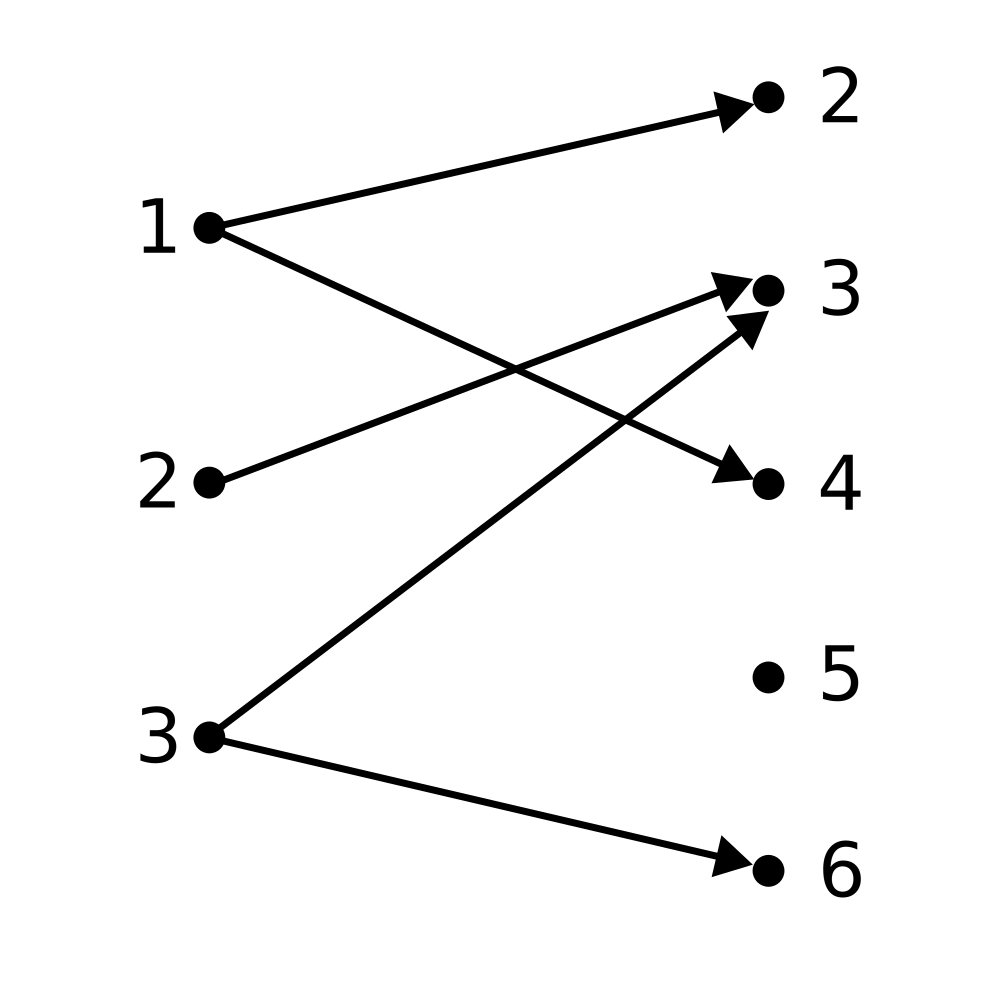
\includegraphics[width=0.5\textwidth]{images/relation-graph.png}
        \caption{Отношение в виде ориентированного графа}
    \end{figure}
\end{example*}

\subsection{Способы задания композиции отношений}

\subsubsection{Матричный способ}

Матрица композиции отношений \(R \circ S\) получается как произведение матриц отношений \(R\) и \(S\) с дальнейшей заменой отличных от нуля элементов единицами.

\begin{example*}
    Пусть
    \begin{gather*}
        R = \{(1, 2), (2, 1), (2, 2), (3, 3), (3, 4)\},
        \\
        S = \{(1, 1), (1, 2), (2, 3), (2, 5), (3, 2), (3, 4), (4, 2), (4, 3)\}.
    \end{gather*}
    Тогда композиция равна
    \begin{gather*}
        [R \circ S] =
        \begin{pmatrix}
            0 & 1 & 0 & 0 \\
            1 & 1 & 0 & 0 \\
            0 & 0 & 1 & 1
        \end{pmatrix}
        \times
        \begin{pmatrix}
            1 & 1 & 0 & 0 & 0 \\
            0 & 0 & 1 & 0 & 1 \\
            0 & 1 & 0 & 1 & 0 \\
            0 & 1 & 1 & 0 & 0
        \end{pmatrix}
        = \\ =
        \begin{pmatrix}
            0 & 0 & 1 & 0 & 1 \\
            1 & 1 & 1 & 0 & 1 \\
            0 & 2 & 1 & 1 & 0
        \end{pmatrix}
        =
        \begin{pmatrix}
            0 & 0 & 1 & 0 & 1 \\
            1 & 1 & 1 & 0 & 1 \\
            0 & 1 & 1 & 1 & 0
        \end{pmatrix}
    \end{gather*}
    \[
        R \circ S = \{(1, 3), (1, 5), (2, 1), (2, 2), (2, 3), (2, 5), (3, 2), (3, 3), (3, 4)\}.
    \]
\end{example*}

\subsubsection{С помощью ориентированного графа}

Пусть \(R \subset A \times B\) и \(S \subset B \times C\). Чтобы получить граф \(T = R \circ S\), надо к графу отношения \(R\) добавить граф отношения \(S\). Граф композиции отношений получим, если исключим вершины, которые являются элементами множества \(B\).

\begin{example*}
    Пусть
    \begin{gather*}
        R = \{(1, 2), (2, 1), (2, 2), (3, 3), (3, 4)\}, \\
        S = \{(1, 1), (1, 2), (2, 3), (2, 5), (3, 2), (3, 4), (4, 2), (4, 3)\}.
    \end{gather*}

    \begin{figure}[H]
        \centering
        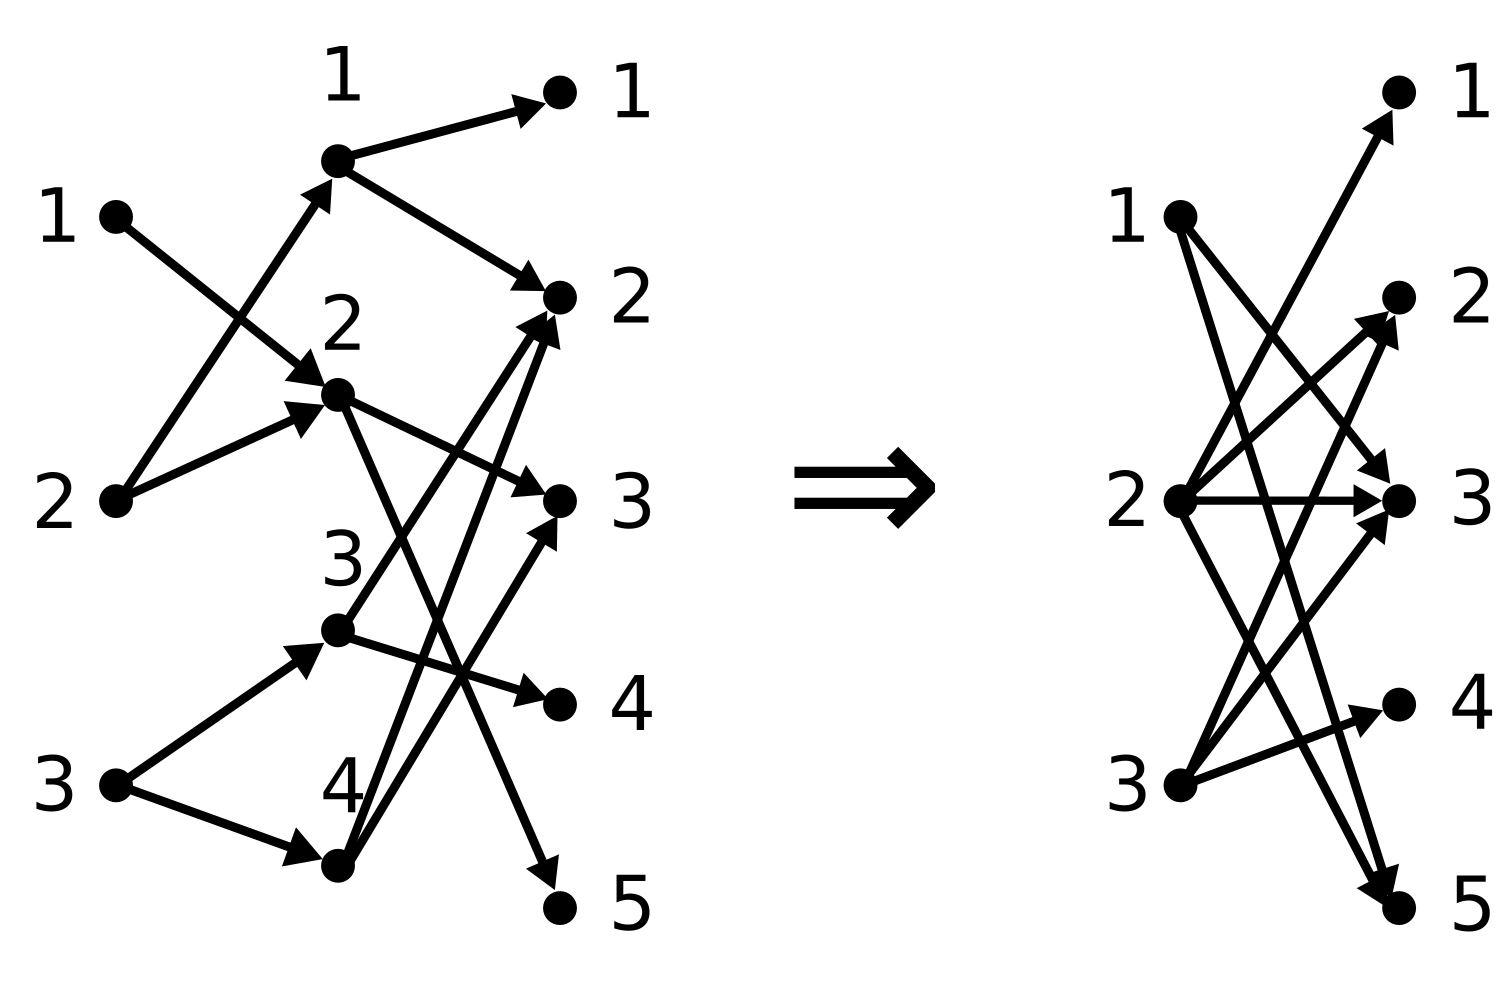
\includegraphics[width=0.8\textwidth]{images/composition-graph.png}
        \caption{Композиция в виде ориентированного графа}
    \end{figure}

    \[
        R \circ S = \{(1, 3), (1, 5), (2, 1), (2, 2), (2, 3), (2, 5), (3, 2), (3, 3), (3, 4)\}.
    \]
\end{example*}

\subsection{Свойства бинарных отношений}

Бинарное отношение \(R\) на множестве \(A\) называется
\begin{itemize}
    \item \textbf{рефлексивным}, если
          \[
              \forall x \in A : (x, x) \in R;
          \]
    \item \textbf{антирефлексивным}, если
          \[
              \forall x \in A : (x, x) \notin R;
          \]
    \item \textbf{симметричным}, если
          \[
              \forall x, y \in A : (x, y) \in R \implies (y, x) \in R ;
          \]
    \item \textbf{антисимметричным}, если
          \[
              \forall x, y \in A : (x, y) \in R \land (y, x) \in R \implies x = y;
          \]
    \item \textbf{транзитивным}, если
          \[
              \forall x, y, z \in A : (x, y) \in R \land (y, z) \in R \implies (x, z) \in R;
          \]
    \item \textbf{линейным} (полным), если
          \[
              \forall x, y \in A : x = y \lor (x, y) \in R \lor (y, x) \in R.
          \]
\end{itemize}

\begin{theorem*}
    Пусть \(R \subset A \times A\) -- отношение на \(A\). Тогда
    \begin{itemize}
        \item \(R \text{ рефлексивно } \iff I \subset R\);
        \item \(R \text{ антирефлексивно } \iff R \cap I = \varnothing\);
        \item \(R \text{ симметрично } \iff R = R^{-1}\);
        \item \(R \text{ антисимметрично } \iff R \cap R^{-1} = I\);
        \item \(R \text{ транзитивно } \iff R \circ R \subset R\);
        \item \(R \text{ линейно } \iff R \cup I \cup R^{-1} = U\).
    \end{itemize}
\end{theorem*}

\subsection{Ядро отношения}

Если \(R \subset A \times B\) -- отношение между множествами \(A\) и \(B\), то композиция \(R \circ R^{-1}\) называется \textbf{ядром} отношения \(R\) и обозначается \(\text{ker} R\):
\[
    \text{ker} R = R \circ R^{-1}.
\]

Ядро отношения \(R\) между \(A\) и \(B\) является отношением на \(A\):
\[
    R \subset A \times B \implies \text{ker} R \subset A^2.
\]

\begin{theorem*}
    Ядро любого отношения рефлексивно и симметрично на области определения.
\end{theorem*}

\subsection{Замыкание отношений}

Пусть \(R\) и \(R^\times\) -- отношения на множестве \(M\). Отношение \(R^\times\) называется замыканием \(R\) относительно свойства \(C\), если
\begin{enumerate}
    \item \(R^\times\) обладает свойством \(C\): \(C(R^\times)\);
    \item \(R^\times\) является надмножеством \(R\): \(R \subset R^\times\);
    \item \(R^\times\) является наименьшим таким объектом:
          \[
              C(R^{\times \times}) \land R \subset R^\times \implies R^\times \subset R^{\times \times}.
          \]
\end{enumerate}

\begin{theorem*}
    Пусть \(R\) -- отношение на множестве \(M\). Тогда
    \begin{itemize}
        \item \(R \cup I\) есть рефлексивное замыкание \(R\);
        \item \(R \cup R^{-1}\) есть симметричное замыкание \(R\);
        \item если \(M\) -- конечное множество, содержащее \(n\) элементов, то отношение
              \[
                  R \cup R^2 \cup R^3 \cup \ldots \cup R^n
              \]
              есть транзитивное замыкание \(R\).
    \end{itemize}
\end{theorem*}

\subsection{Функциональные отношения}

Пусть \(f\) -- отношение между \(A\) и \(B\) такое, что
\[
    \forall a : (a, b) \in f \land (a, c) \in f \implies b = c.
\]

Такое свойство отношений называется \textbf{однозначностью} или \textbf{функциональным}, а само отношение называется \textbf{функцией} из \(A\) в \(B\).
\[
    f: A \to B \quad \text{или} \quad A \stackrel{f}{\to} B.
\]

\[
    b = f(a) \iff (a, b) \in f.
\]

\subsection{Тотальные и частичные функции}

\[
    \text{Dom} f \subset A;
    \qquad
    \text{Im} f \subset B
\]

Если \(\text{Dom} f = A\), то функция называется \textbf{тотальной}, а если \(\text{Dom} f \neq A\), то \textbf{частичной}.

\subsection{Инъекция, сюрьекция и биекция}

Пусть \(f: A \to B\), тогда функция \(f\) называется
\begin{itemize}
    \item \textbf{инъективной} (или инъекцией), если
          \[
              b = f(a_1) \land b = f(a_2) \implies a_1 = a_2;
          \]
    \item \textbf{сюрьективной} (или сюрьекцией), если
          \[
              \forall b \in B \; \exists a \in A : b = f(a);
          \]
    \item \textbf{биективной} (или биекцией), если она инъективная и сюрьективная.
\end{itemize}

\subsection{Отношения эквивалентности}

Отношение называется отношением \textbf{эквивалентности} (эквивалентностью), если оно рефлексивно, симметрично и транзитивно. Эквивалентности обозначают символами \(E\), \(\sim\) (тильда) и \(=\):
\[
    xEy,
    \quad
    x \sim y,
    \quad
    x = y.
\]

\begin{example*}
    Отношение равенства \(x = y\) является эквивалентностью на любом множестве \(A\), так как оно
    \begin{itemize}
        \item рефлексивно (\(x = x\));
        \item симметрично (\(x = y \implies y = x\));
        \item транзитивно (\(x = y, y = z \implies x = z\)).
    \end{itemize}
\end{example*}


\subsection{Классы эквивалентности}

Пусть \(E\) -- отношение эквивалентности на множестве \(A\). \textbf{Классом эквивалентности} элемента \(x \in A\) называется подмножество элементов множества \(A\), эквивалентных \(x\):
\begin{gather*}
    E(x) = \{y \in A \mid xEy\}
    \\ \text{или} \\
    [x]_E = \{y \in A \mid y \equiv x\}.
\end{gather*}

\subsection{Фактормножества}

Если \(E\) -- отношение эквивалентности на множестве \(A\), то множество классов эквивалентности называется \textbf{фактормножеством} множества \(A\) относительно эквивалентности \(E\) и обозначается \(A \slash E\):
\[
    A \slash E = \{E(x) \mid x \in A\}
    \quad
    \text{или}
    \quad
    A \slash E = \{[x]_E\}_{x \in A}.
\]

\subsection{Отношения порядка}

Антисимметричное транзитивное отношение называется \textbf{отношением порядка}. Отношение порядка в общем случае обозначается символом \(\prec\). Отношение порядка может обладать также дополнительными свойствами, которые сведены в следующую таблицу:

\begin{center}
    \renewcommand*{\arraystretch}{1.5}
    \begin{longtable}{|C{0.45\textwidth}|C{0.45\textwidth}|}
        \hline
        Дополнительное свойство, которым обладает отношением порядка & Название отношения порядка, обладающего дополнительным свойством \\
        \hline
        рефлексивность                                               & отношение нестрогого порядка \(\leq\)                            \\
        \hline
        антирефлексивность                                           & отношение строгого порядка \(<\)                                 \\
        \hline
        линейность                                                   & отношение линейного порядка                                      \\
        \hline
        не обладает свойством линейности                             & отношение частичного порядка                                     \\
        \hline
    \end{longtable}
\end{center}

Множества, на котором задано отношение частичного порядка, называется \textbf{частично упорядоченным}.

Множество, на котором задано отношение линейного порядка, называется \textbf{линейно упорядоченным}.

\section{Элементы математической логики}

\subsection{Основные понятия}

\textbf{Математическая логика} -- это анализ методом рассуждений, при этом в первую очередь исследуются формы рассуждений, а не их содержание, т. е. математическая логика исследует соотношения между основными понятиями математики, на базе которых доказываются математические утверждения.

Простейшую из формальных логических теорий называют \textbf{алгеброй высказываний}.

\textbf{Высказыванием} называется утверждение (повествовательное предложение), о котором в данной ситуации можно сказать, что оно истинно или ложно, но не то и другое одновременно.

Высказыванию ставят в соответствие логическую переменную, которая принимает значение \(1\), если высказывание истинно, и \(0\), если высказывание ложно.

Из простых высказываний с помощью \textbf{логических связок} могут быть построены \textbf{составные высказывания}.

\subsection{Логические связки}

\subsubsection{Простейшие логические связки}

В таблице \ref{tab:simplest-logical-connectives} представлены простейшие логические связки.

{
\renewcommand*{\arraystretch}{1.5}
\begin{longtable}{|c|c|c|}
    \hline
    \textbf{Название} & \textbf{Прочтение}          & \textbf{Обозначение} \\
    \hline
    отрицание         & не                          & \(\lnot\)            \\
    \hline
    конъюнкция        & и                           & \(\land\)            \\
    \hline
    дизъюнкция        & или                         & \(\lor\)             \\
    \hline
    импликация        & если, то                    & \(\to\)              \\
    \hline
    эквивалентность   & тогда и только тогда, когда & \(\leftrightarrow\)  \\
    \hline
    \caption{Простейшие логические связки}
    \label{tab:simplest-logical-connectives}
\end{longtable}
}

Таблица \ref{tab:truth-table-slc} представляет собой таблицу истинности простейших логических связок.

{
\renewcommand*{\arraystretch}{1.5}
\begin{longtable}{|c|c|c|c|c|c|c|}
    \hline
    \(A\) & \(B\) & \(\bar{A}\) & \(A \land B\) & \(A \lor B\) & \(A \to B\) & \(A \leftrightarrow B\) \\
    \hline
    \(0\) & \(0\) & \(1\)       & \(0\)         & \(0\)        & \(1\)       & \(1\)                   \\
    \hline
    \(0\) & \(1\) & \(1\)       & \(0\)         & \(1\)        & \(1\)       & \(0\)                   \\
    \hline
    \(1\) & \(0\) & \(0\)       & \(0\)         & \(1\)        & \(0\)       & \(0\)                   \\
    \hline
    \(1\) & \(1\) & \(0\)       & \(1\)         & \(1\)        & \(1\)       & \(1\)                   \\
    \hline
    \caption{Таблица истинности простейших логических связок}
    \label{tab:truth-table-slc}
\end{longtable}
}


\subsubsection{Порядок выполнения логических операций}

Если скобок нет, то операции выполняются в следующем порядке:
\begin{enumerate}
    \item отрицание;
    \item конъюнкция;
    \item дизъюнкция;
    \item импликация;
    \item эквивалентность.
\end{enumerate}

\subsubsection{Доказательство тождественной истинности}

\begin{example*}
    Необходимо доказать тождественную истинность формулы
    \[
        \bar{A} \to (A \to B).
    \]

    {
    \renewcommand*{\arraystretch}{1.5}
    \begin{longtable}{|c|c|c|c|c|}
        \hline
        \(A\) & \(B\) & \(\bar{A}\) & \(A \to B\) & \(\bar{A} \to (A \to B)\) \\
        \hline
        \(0\) & \(0\) & \(1\)       & \(1\)       & \(1\)                     \\
        \hline
        \(0\) & \(1\) & \(1\)       & \(1\)       & \(1\)                     \\
        \hline
        \(1\) & \(0\) & \(0\)       & \(0\)       & \(1\)                     \\
        \hline
        \(1\) & \(1\) & \(0\)       & \(1\)       & \(1\)                     \\
        \hline
        \caption{Пример доказательства тождественной истинности}
    \end{longtable}
    }
\end{example*}

\subsubsection{Другие логические связки}

В таблице \ref{tab:other-logical-connectives} представлены другие логические связки, которые мы в дальнейшем будем использовать.

{
\renewcommand*{\arraystretch}{1.5}
\begin{longtable}{|c|c|c|}
    \hline
    \textbf{Название}   & \textbf{Прочтение}  & \textbf{Обозначение} \\
    \hline
    Штрих Шеффера       & антиконъюнкция      & \(|\)                \\
    \hline
    Стрелка Пирса       & антидизъюнкция      & \(\downarrow\)       \\
    \hline
    Сумма по модулю два & антиэквивалентность & \(\oplus\)           \\
    \hline
    \caption{Другие логические связки}
    \label{tab:other-logical-connectives}
\end{longtable}
}

Эти логические связки можно представить следующим образом:
\[
    A \mathop{|} B = \overline{A \land B};
    \quad
    A \downarrow B = \overline{A \lor B};
    \quad
    A \oplus B = \overline{A \leftrightarrow B}.
\]

Таблица \ref{tab:truth-table-olc} представляет собой таблицу истинности других логических связок.

{
\renewcommand*{\arraystretch}{1.5}
\begin{longtable}{|c|c|c|c|c|}
    \hline
    \(A\) & \(B\) & \(A \mathop{|} B\) & \(A \downarrow B\) & \(A \oplus B\) \\
    \hline
    \(0\) & \(0\) & \(1\)              & \(1\)              & \(0\)          \\
    \hline
    \(0\) & \(1\) & \(1\)              & \(0\)              & \(1\)          \\
    \hline
    \(1\) & \(0\) & \(1\)              & \(0\)              & \(1\)          \\
    \hline
    \(1\) & \(1\) & \(0\)              & \(0\)              & \(0\)          \\
    \hline
    \caption{Таблица истинности других логических связок}
    \label{tab:truth-table-olc}
\end{longtable}
}

\begin{note*}
    Таблицы истинности содержат \(2^n\) строк, где \(n\) -- число простых логических высказываний.
\end{note*}

\subsection{Логические отношения}

Отношение следствия: из \(A\) следует \(B\), если \(B\) истинно всякий раз, когда истинно \(A\).

\begin{example*}
    Рассмотрим высказывания \(A \leftrightarrow B\), \(A \to B\), \(A \lor B\):
    {
    \renewcommand*{\arraystretch}{1.5}
    \begin{longtable}{|c|c|c|c|c|}
        \hline
        \(A\) & \(B\) & \(A \leftrightarrow B\) & \(A \to B\) & \(A \lor B\) \\
        \hline
        \(0\) & \(0\) & \(1\)                   & \(1\)       & \(0\)        \\
        \hline
        \(0\) & \(1\) & \(0\)                   & \(1\)       & \(1\)        \\
        \hline
        \(1\) & \(0\) & \(0\)                   & \(0\)       & \(1\)        \\
        \hline
        \(1\) & \(1\) & \(1\)                   & \(1\)       & \(1\)        \\
        \hline
    \end{longtable}
    }
    Из \(A \leftrightarrow B\) следует \(A \to B\), однако из \(A \leftrightarrow B\) не следует \(A \lor B\).
\end{example*}

Два составных высказывания \textbf{эквивалентны}, если они имеют одинаковые истинностные значения на одинаковых наборах, т. е. последние столбцы их таблиц истинности должны совпадать.

\begin{example*}
    Проверим, являются ли высказывания \(A \to B\) и \(\bar{A} \lor B\) эквивалентными:

    \begin{minipage}[c]{0.5\textwidth}
        \renewcommand*{\arraystretch}{1.5}
        \begin{longtable}{|c|c|c|}
            \hline
            \(A\) & \(B\) & \(A \to B\) \\
            \hline
            \(0\) & \(0\) & \(1\)       \\
            \hline
            \(0\) & \(1\) & \(1\)       \\
            \hline
            \(1\) & \(0\) & \(0\)       \\
            \hline
            \(1\) & \(1\) & \(1\)       \\
            \hline
        \end{longtable}
    \end{minipage}
    \begin{minipage}[c]{0.5\textwidth}
        \renewcommand*{\arraystretch}{1.5}
        \begin{longtable}{|c|c|c|c|}
            \hline
            \(A\) & \(B\) & \(\bar{A}\) & \(\bar{A} \lor B\) \\
            \hline
            \(0\) & \(0\) & \(1\)       & \(1\)              \\
            \hline
            \(0\) & \(1\) & \(1\)       & \(1\)              \\
            \hline
            \(1\) & \(0\) & \(0\)       & \(0\)              \\
            \hline
            \(1\) & \(1\) & \(0\)       & \(1\)              \\
            \hline
        \end{longtable}
    \end{minipage}

    \vspace*{1em}

    Итого получим, что
    \[
        A \to B \equiv \bar{A} \lor B.
    \]
\end{example*}

\subsection{Варианты импликации}

\textbf{Импликация} двух высказываний отличается от эквивалентности, а также от дизъюнкции и конъюнкции тем, что она \textbf{несимметрична} (т. е. \(A \to B\) не эквивалентно \(B \to A\)).

Для высказывания \(A \to B\):
\begin{itemize}
    \item высказывание \(B \to A\) называется \textbf{конверсией};
    \item высказывание \(\bar{A} \to \bar{B}\) называется \textbf{конверсией контрапозиции};
    \item высказывание \(\bar{B} \to \bar{A}\) называется \textbf{контрапозицией}.
\end{itemize}

Таблица \ref{tab:truth-table-implication} представляет собой таблицу истинности этих вариантов импликации.

{
\renewcommand*{\arraystretch}{1.5}
\begin{longtable}{|c|c|c|c|c|c|c|c|}
    \hline
    \(A\) & \(B\) & \(\bar{A}\) & \(\bar{B}\) & \(A \to B\) & \(B \to A\) & \(\bar{A} \to \bar{B}\) & \(\bar{B} \to \bar{A}\) \\
    \hline
    \(0\) & \(0\) & \(1\)       & \(1\)       & \(1\)       & \(1\)       & \(1\)                   & \(1\)                   \\
    \hline
    \(0\) & \(1\) & \(1\)       & \(0\)       & \(1\)       & \(0\)       & \(0\)                   & \(1\)                   \\
    \hline
    \(1\) & \(0\) & \(0\)       & \(1\)       & \(0\)       & \(1\)       & \(1\)                   & \(0\)                   \\
    \hline
    \(1\) & \(1\) & \(0\)       & \(0\)       & \(1\)       & \(1\)       & \(1\)                   & \(1\)                   \\
    \hline
    \caption{Таблица истинности вариантов импликации}
    \label{tab:truth-table-implication}
\end{longtable}
}

\subsection{Необходимое и достаточное условия}

{
    \renewcommand*{\arraystretch}{1.5}
    \begin{longtable}{|C{0.27\textwidth}|C{0.27\textwidth}|C{0.27\textwidth}|}
        \hline
        \textbf{Условие}                                            & \textbf{Описание}                                               & \textbf{Операция}                                                 \\
        \hline
        \(A\) является достаточным условием для \(B\)               & Если имеет место \(A\), то \(B\) также будет иметь место        & Импликация \(A \to B\)                                            \\
        \hline
        \(A\) является необходимым условием для \(B\)               & Если имеет место \(B\), то \(A\) также будет иметь место        & Конверсия достаточного условия \(B \to A\)                        \\
        \hline
        \(A\) является необходимым и достаточным условием для \(B\) & \(A\) имеет место тогда и только тогда, когда имеет место \(B\) & Двойная импликация, т. е. эквивалентность \(A \leftrightarrow B\) \\
        \hline
    \end{longtable}
}

\subsection{Основные логические эквивалентности}

\begin{property}[Идемпотентность]
    \[
        A \lor A = A,
        \quad
        A \land A = A.
    \]
\end{property}

\begin{property}[Коммутативность]
    \[
        A \lor B = B \lor A,
        \quad
        A \land B = B \land A.
    \]
\end{property}

\begin{property}[Ассоциативность]
    \[
        A \lor (B \lor C) = (A \lor B) \lor C,
        \quad
        A \land (B \land C) = (A \land B) \land C.
    \]
\end{property}

\begin{property}[Дистрибутивность]
    \[
        A \lor (B \land C) = (A \lor B) \land (A \lor C),
        \quad
        A \land (B \lor C) = (A \land B) \lor (A \land C).
    \]
\end{property}

\begin{property}[Поглощение]
    \[
        (A \land B) \lor A = A,
        \quad
        (A \lor B) \land A = A.
    \]
\end{property}

\begin{property}[Свойства нуля]
    \[
        A \lor 0 = A,
        \quad
        A \land 0 = 0.
    \]
\end{property}

\begin{property}[Свойства единицы]
    \[
        A \lor 1 = 1,
        \quad
        A \land 1 = A.
    \]
\end{property}

\begin{property}[Инволютивность]
    \[
        \bar{\bar{A}} = A.
    \]
\end{property}

\begin{property}[Законы де Моргана]
    \[
        \overline{A \land B} = \bar{A} \lor \bar{B},
        \quad
        \overline{A \lor B} = \bar{A} \land \bar{B}.
    \]
\end{property}

\begin{property}[Свойства дополнения]
    \[
        A \lor \bar{A} = 1,
        \quad
        A \land \bar{A} = 0.
    \]
\end{property}

\begin{property}[Свойство импликации]
    \[
        A \to B = \bar{A} \lor B.
    \]
\end{property}

\begin{property}[Свойство эквивалентности]
    \[
        A \leftrightarrow B = (A \to B) \land (B \to A).
    \]
\end{property}

\subsection{Булевы функции}

\textbf{Булевы функции} находят применение в конструировании и упрощении логических схем.

Обозначим \(E_2 = \{0, 1\}\), тогда
\[
    E_2^n = \underbrace{E_2 \times E_2 \times \ldots \times E_2}_{n}.
\]

Функции \(f: E_2^n \to E_2\) называются \textbf{функции алгебры логики} или \textbf{булевыми функциями} от \(n\) переменных. Множество булевых функций от \(n\) переменных обозначают \(P_n\):
\[
    P_n = \{f \mid f : E_2^n \to E_2\}.
\]

\subsection{Множество булевых функций. Булев куб}

\(P_2\) -- множество всех булевых функций.

\(P_{2, n}\) -- множество всех булевых функций от \(n\) переменных:
\[
    P_{2, n} = \{f \mid f : E_2^n \to E_2\},
    \qquad
    P_2 = \bigcup_{n \geq 0} P_{2, n}.
\]

\(\{0, 1\}^n\) -- \textbf{булев куб} размерности \(n\). Число всех элементов булева куба \(\{0, 1\}^n\) составляет \(2^n\).

\subsection{Булев порядок}

Для произвольных наборов \(\bar{\alpha} = (\alpha_1, \ldots, \alpha_n)\) и \(\bar{\beta} = (\beta_1, \ldots, \beta_n)\) имеет место
\[
    \bar{\alpha} \leq \bar{\beta}
    \iff
    \alpha_i \leq \beta_i,
    \forall i = \overline{1, n}
\]
то есть
\[
    \bar{\alpha} \leq \bar{\beta}
    \iff
    \alpha_i = \beta_i
    \text{ или }
    \alpha_i, \beta_i = 1, \forall i = \overline{1, n}.
\]

Если существует хотя бы одно \(i\), для которого \(\alpha_i = 0\), \(\beta_i = 1\), то имеет место строгое неравенство \(\bar{\alpha} < \bar{\beta}\).

Если существует ровно одно \(i\), для которого \(\alpha_i = 0\), \(\beta_i = 1\), то набор \(\bar{\beta}\) \textbf{доминирует} над набором \(\bar{\alpha}\).

Рассмотренное отношение порядка на \(B^n\), где \(B^n\) -- \(n\)-я декартова степень
\[
    B = (\{0, 1\}, \lor, \land, 0, 1)
\]
будем называть \textbf{булевым порядком}.

Булев куб как упорядоченное множество можно изобразить в виде диаграммы Хассе
\begin{figure}[H]
    \centering
    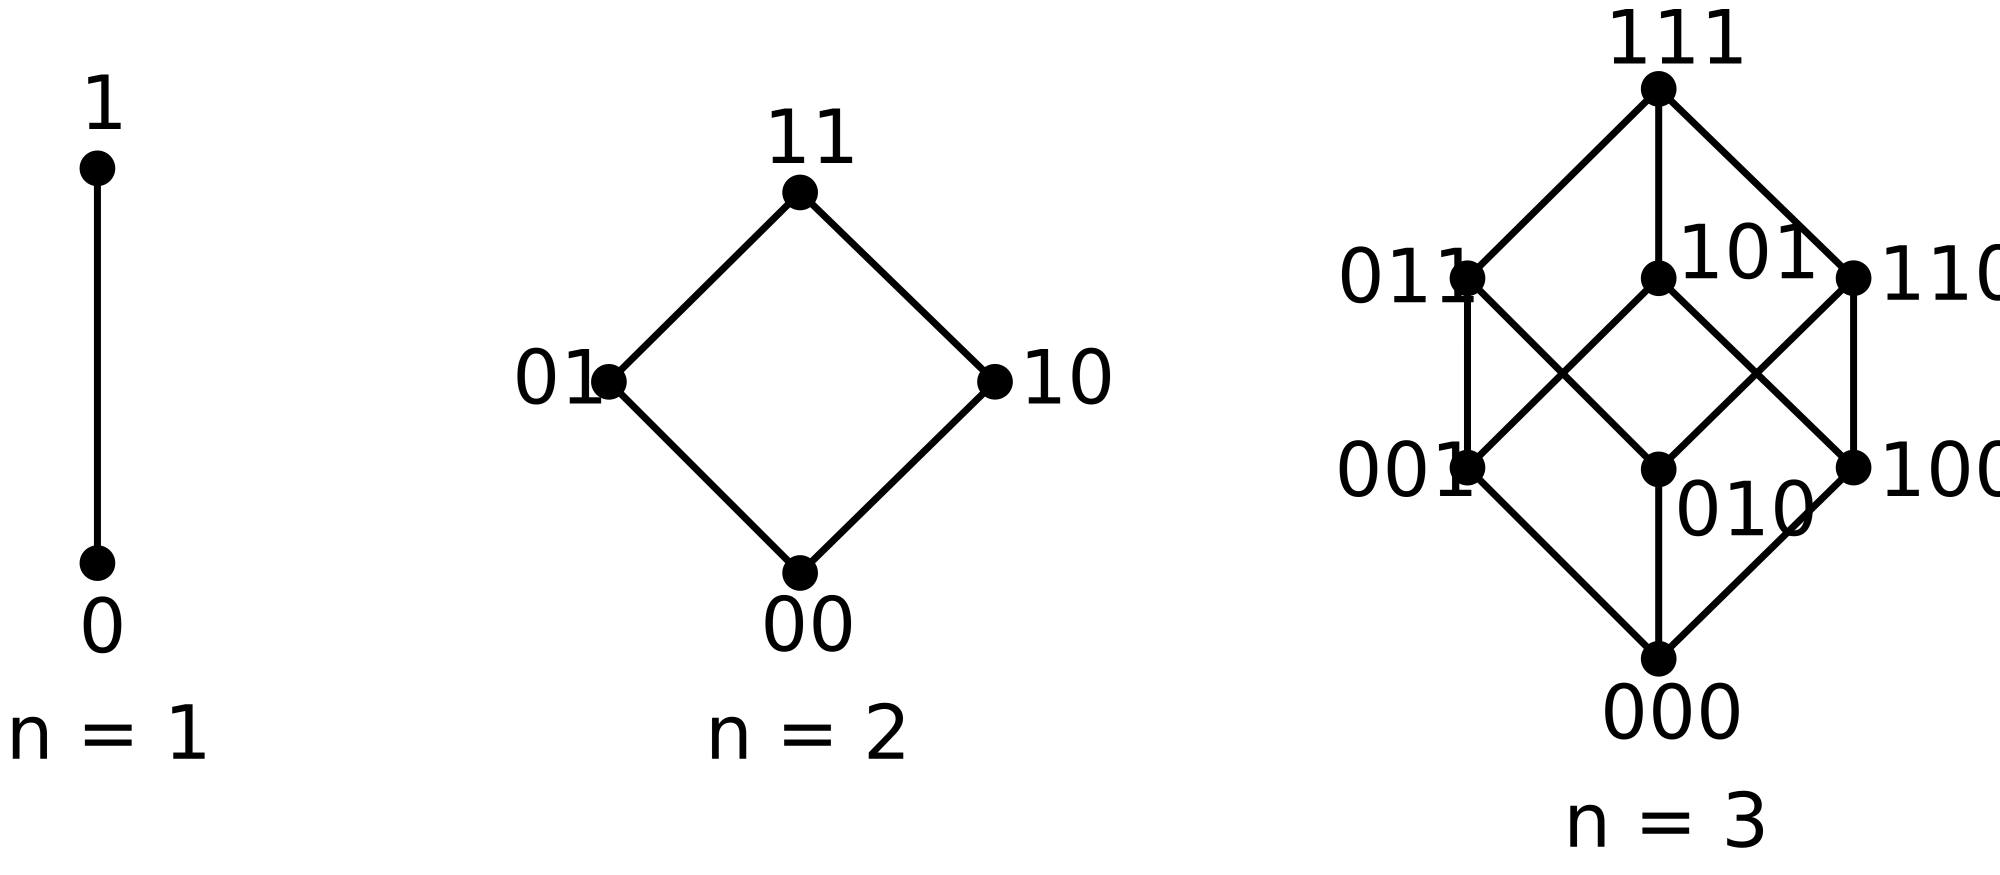
\includegraphics[width=0.9\textwidth]{images/boolean-cube.png}
    \caption{Примеры булевых кубов в виде диаграммы Хассе}
\end{figure}

\subsection{Мощность множества булевых функций}

\textbf{Число булевых функций} от \(n\) переменных находится по формуле
\[
    |P_{2, n}| = 2^{2^n}.
\]

{
\renewcommand*{\arraystretch}{1.5}
\begin{longtable}{|c|c|c|c|c|}
    \hline
    \(x_1\)    & \(\ldots\) & \(x_{n - 1}\) & \(x_n\)    & \(f(x_1, \ldots x_n)\) \\
    \hline
    \(0\)      & \(\ldots\) & \(0\)         & \(0\)      & \(f(0, \ldots, 0, 0)\) \\
    \hline
    \(0\)      & \(\ldots\) & \(0\)         & \(1\)      & \(f(0, \ldots, 0, 1)\) \\
    \hline
    \(0\)      & \(\ldots\) & \(1\)         & \(0\)      & \(f(0, \ldots, 1, 0)\) \\
    \hline
    \(\ldots\) & \(\ldots\) & \(\ldots\)    & \(\ldots\) & \(\ldots\)             \\
    \hline
    \(1\)      & \(\ldots\) & \(1\)         & \(1\)      & \(f(1, \ldots, 1, 1)\) \\
    \hline
    \caption{Таблица булевых функций}
\end{longtable}
}

\subsection{Существенные и несущественные переменные}

Булева функция \(f \in P_n\) \textbf{существенно зависит} от переменной \(x_i\), если существует такой набор значений
\[
    a_1, \ldots, a_{i - 1}, a_{i +1}, \ldots, a_n
\]

что
\[
    f(a_1, \ldots, a_{i - 1}, 0, a_{i +1}, \ldots, a_n) \neq f(a_1, \ldots, a_{i - 1}, 0, a_{i +1}, \ldots, a_n).
\]

В этом случае \(x_i\) называют \textbf{существенной} переменной, в противном случае \(x_i\) называют \textbf{несущественной} (фиктивной) переменной.

\begin{example*}
    Рассмотрим следующую таблицу истинности:

    \vspace*{1em}

    {
        \renewcommand*{\arraystretch}{1.5}
        \begin{longtable}{|c|c|c|c|}
            \hline
            \(x_1\) & \(x_2\) & \(f_1\) & \(f_2\) \\
            \hline
            \(0\)   & \(0\)   & \(0\)   & \(1\)   \\
            \hline
            \(0\)   & \(1\)   & \(0\)   & \(1\)   \\
            \hline
            \(1\)   & \(0\)   & \(1\)   & \(0\)   \\
            \hline
            \(1\)   & \(1\)   & \(1\)   & \(0\)   \\
            \hline
        \end{longtable}
    }

    В данном случае \(x_1\) -- существенная переменная, а \(x_2\) -- несущественная, поскольку
    \begin{gather*}
        f_1(0, 0) = f_1(0, 1),
        \quad
        f_1(1, 0) = f_1(1, 1).
        \\
        f_2(0, 0) = f_2(0, 1),
        \quad
        f_2(1, 0) = f_2(1, 1).
    \end{gather*}
\end{example*}

\subsection{Булевы функции одной и нескольких переменной}

{
    \renewcommand*{\arraystretch}{1.5}
    \begin{longtable}{|c|c|c|c|c|}
        \hline
        \(x\) & \(f_1\) & \(f_2\) & \(f_3\) & \(f_4\) \\
        \hline
        \(0\) & \(0\)   & \(0\)   & \(1\)   & \(1\)   \\
        \hline
        \(1\) & \(0\)   & \(1\)   & \(0\)   & \(1\)   \\
        \hline
        \caption{Булевы функции одной переменной}
    \end{longtable}
}

{
    \setlength{\tabcolsep}{3pt}
    \renewcommand*{\arraystretch}{1.5}
    \begin{longtable}{|c|c!{\vrule width 1.2pt}Sc|c|c|c|c|c|c|c|c|c|c|c|c|c|c|c|c|}
        \hline
        \(x_1\) & \(x_2\) & \(f_1\) & \(f_2\) & \(f_3\) & \(f_4\) & \(f_5\) & \(f_6\) & \(f_7\) & \(f_8\) & \(f_9\) & \(f_{10}\) & \(f_{11}\) & \(f_{12}\) & \(f_{13}\) & \(f_{14}\) & \(f_{15}\) & \(f_{16}\) \\
        \hline
        \(0\)   & \(0\)   & \(0\)   & \(0\)   & \(0\)   & \(0\)   & \(0\)   & \(0\)   & \(0\)   & \(0\)   & \(1\)   & \(1\)      & \(1\)      & \(1\)      & \(1\)      & \(1\)      & \(1\)      & \(1\)      \\
        \hline
        \(0\)   & \(1\)   & \(0\)   & \(0\)   & \(0\)   & \(0\)   & \(1\)   & \(1\)   & \(1\)   & \(1\)   & \(0\)   & \(0\)      & \(0\)      & \(0\)      & \(1\)      & \(1\)      & \(1\)      & \(1\)      \\
        \hline
        \(1\)   & \(0\)   & \(0\)   & \(0\)   & \(1\)   & \(1\)   & \(0\)   & \(0\)   & \(1\)   & \(1\)   & \(0\)   & \(0\)      & \(1\)      & \(1\)      & \(0\)      & \(0\)      & \(1\)      & \(1\)      \\
        \hline
        \(1\)   & \(1\)   & \(0\)   & \(1\)   & \(0\)   & \(1\)   & \(0\)   & \(1\)   & \(0\)   & \(1\)   & \(0\)   & \(1\)      & \(0\)      & \(1\)      & \(0\)      & \(1\)      & \(0\)      & \(1\)      \\
        \hline
        \caption{Булевы функции двух переменных}
    \end{longtable}
}

\subsection{Мажоритарная функция}

{
    \renewcommand*{\arraystretch}{1.5}
    \begin{longtable}{|c|c|c|c|c|}
        \hline
              & \(x_1\) & \(x_2\) & \(x_3\) & \(f(x_1, x_2, x_3)\) \\
        \hline
        \(0\) & \(0\)   & \(0\)   & \(0\)   & \(0\)                \\
        \hline
        \(1\) & \(0\)   & \(0\)   & \(1\)   & \(0\)                \\
        \hline
        \(2\) & \(0\)   & \(1\)   & \(0\)   & \(0\)                \\
        \hline
        \(3\) & \(0\)   & \(1\)   & \(1\)   & \(1\)                \\
        \hline
        \(4\) & \(1\)   & \(0\)   & \(0\)   & \(0\)                \\
        \hline
        \(5\) & \(1\)   & \(0\)   & \(1\)   & \(1\)                \\
        \hline
        \(6\) & \(1\)   & \(1\)   & \(0\)   & \(1\)                \\
        \hline
        \(7\) & \(1\)   & \(1\)   & \(1\)   & \(1\)                \\
        \hline
        \caption{Мажоритарная функция (функция голосования)}
    \end{longtable}
}

\subsection{Реализация функций формулами}

Так же, как составные высказывания строятся из более простых, с помощью логических операций, можно комбинировать булевы переменные с помощью булевых операций, получая булевы выражения, которые называются \textbf{формулами}. Всякой формуле однозначно соответствует некоторая функция, при этом говорят, что \textbf{формула реализует функцию}.

\begin{example*}
    Построим таблицу истинности для формулы
    \[
        ((x_1 \land x_2) \oplus x_1) \oplus x_2.
    \]

    {
    \renewcommand*{\arraystretch}{1.5}
    \begin{longtable}{|c|c|c|c|c|}
        \hline
        \(x_1\) & \(x_2\) & \(x_1 \land x_2\) & \((x_1 \land x_2) \oplus x_1\) & \(((x_1 \land x_2) \oplus x_1) \oplus x_2\) \\
        \hline
        \(0\)   & \(0\)   & \(0\)             & \(0\)                          & \(0\)                                       \\
        \hline
        \(0\)   & \(1\)   & \(0\)             & \(0\)                          & \(1\)                                       \\
        \hline
        \(1\)   & \(0\)   & \(0\)             & \(1\)                          & \(1\)                                       \\
        \hline
        \(1\)   & \(1\)   & \(1\)             & \(0\)                          & \(1\)                                       \\
        \hline
    \end{longtable}
    }

    Формула \(((x_1 \land x_2) \oplus x_1) \oplus x_2\) реализует функцию \(f_8(x_1, x_2) = 0111\).
\end{example*}

\subsection{Равносильные формулы}

Одна функция может иметь множество реализацией. Формулы, реализующие одну и ту же функцию, называются \textbf{равносильными}:
\[
    \mathcal{F}_1 = \mathcal{F}_2
    \iff
    \exists f: \text{func} \; \mathcal{F}_1 = f \land \text{func} \; \mathcal{F}_2 = f.
\]

Другими словами, булевы функции \(f\) и \(g\) называют равносильными, если их существенные переменные соответственно равны и на каждом наборе значений этих переменных функции \(f\) и \(g\) принимают равные значения.

\begin{example*}
    Пусть
    \[
        f(x, y) = x \lor y,
        \quad
        g(x, y, z) = xz \lor x \bar{z} \lor yz \lor y \bar{z}.
    \]

    Упростим функцию \(g(x, y, z)\):
    \[
        g(x, y, z) =
        xz \lor x \bar{z} \lor yz \lor y \bar{z} =
        x(z \lor \bar{z}) \lor y(z \lor \bar{z}) =
        x \lor y.
    \]

    Получили, что функции \(f(x, y)\) и \(g(x, y, z)\) равносильны.
\end{example*}

\subsection{Законы булевой алгебры}

\begin{property}[Идемпотентность]
    \[
        a \lor a = a,
        \quad
        a \land a = a.
    \]
\end{property}

\begin{property}[Коммутативность]
    \[
        a \lor b = b \lor a,
        \quad
        a \land b = b \land a.
    \]
\end{property}

\begin{property}[Ассоциативность]
    \[
        a \lor (b \lor c) = (a \lor b) \lor c,
        \quad
        a \land (b \land c) = (a \land b) \land c.
    \]
\end{property}

\begin{property}[Дистрибутивность]
    \[
        a \lor (b \land c) = (a \lor b) \land (a \lor c),
        \quad
        a \land (b \lor c) = (a \land b) \lor (a \land c).
    \]
\end{property}

\begin{property}[Поглощение]
    \[
        (a \land b) \lor a = a,
        \quad
        (a \lor b) \land a = a.
    \]
\end{property}

\begin{property}[Свойства нуля]
    \[
        a \lor 0 = a,
        \quad
        a \land 0 = 0.
    \]
\end{property}

\begin{property}[Свойства единицы]
    \[
        a \lor 1 = 1,
        \quad
        a \land 1 = a.
    \]
\end{property}

\begin{property}[Инволютивность]
    \[
        \bar{\bar{a}} = a.
    \]
\end{property}

\begin{property}[Законы де Моргана]
    \[
        \overline{a \land b} = \bar{a} \lor \bar{b},
        \quad
        \overline{a \lor b} = \bar{a} \land \bar{b}.
    \]
\end{property}

\begin{property}[Свойства дополнения]
    \[
        a \lor \bar{a} = 1,
        \quad
        a \land \bar{a} = 0.
    \]
\end{property}

\begin{property}[Свойство импликации]
    \[
        a \to b = \bar{a} \lor b.
    \]
\end{property}

\begin{property}[Свойство эквивалентности]
    \[
        a \leftrightarrow b = (a \to b) \land (b \to a).
    \]
\end{property}

\subsection{Двойственная функция}

Пусть \(f(x_1, \ldots, x_n) \in P_n\) -- булева функция. Тогда функция
\[
    f^*(x_1, \ldots, x_n) = \overline{f(\bar{x}_1, \ldots, \bar{x}_n)}
\]
называется \textbf{двойственной} к функции \(f\).

\begin{example}
    \[
        0^* = \bar{0} = 1.
    \]
\end{example}

\begin{example}
    \[
        1^* = \bar{1} = 0.
    \]
\end{example}

\begin{example}
    \[
        x^* = \bar{\bar{x}} = x.
    \]

    Т. к. \(x\) в данном случае и функция, и переменная, мы применяем двойное отрицание.
\end{example}

\begin{example}
    \[
        (x \land y)^* = \overline{\bar{x} \land \bar{y}} = x \lor y.
    \]
\end{example}

\begin{example}
    \[
        (x \lor y)^* = \overline{\bar{x} \lor \bar{y}} = x \land y.
    \]
\end{example}

\subsection{Инволютивность двойственности}

Из определения видно, что двойственность инволютивна: \(f^{**} = f\), поэтому отношение <<быть двойственной к>> на множестве булевых функций симметрично, то есть, если \(f^* = g\), то \(g^* = f\).

Если в таблице истинности булевой функции \(f\) инвертировать все значения, то получим таблицу истинности двойственной функции \(f^*\).

\subsection{Самодвойственная функция}

Функция называется \textbf{самодвойственной}, если \(f^* = f\). Примером такой функции может служить функция \(f(x) = x\):
\[
    x^* = \bar{\bar{x}} = x.
\]

\subsection{Принцип двойственности}

\begin{theorem*}
    Пусть \(F = \{f_1, \ldots, f_m\}\) -- система булевых функций, а \(F^* = \{f_1^*, \ldots, f_n^*\}\) -- система двойственных функций. Тогда если формула \(\mathcal{F}\) над базисом \(F\) реализует функцию \(f\), то формула \(\mathcal{F}^*\) над базисом \(F^*\), полученная заменой функций \(f_i\), двойственными функциями \(f_i^*\), реализует функцию \(f^*\):
    \[
        \text{func} \; \mathcal{F} |F| = f
        \implies
        \text{func} \; \mathcal{F}^* |F^*| = f^*.
    \]

    \begin{consequence*}
        Если две равносильные формулы заменить двойственными, то равносильность сохранится:
        \[
            \mathcal{F}_1 = \mathcal{F}_2
            \implies
            \mathcal{F}_1^* = \mathcal{F}_2^*.
        \]
    \end{consequence*}
\end{theorem*}

\begin{note*}
    Формула, двойственная к булевой формуле, может быть получена заменой констант \(0\) на \(1\), \(1\) на \(0\), операций \(\land\) на \(\lor\), \(\lor\) на \(\land\) и сохранением структуры формулы.
\end{note*}

\subsection{Нормальные формы}

Если \(x\) -- логическая переменная, \(\sigma \in \{0, 1\}\), то выражение
\[
    x^\sigma =
    \begin{dcases}
        x, \text{если } \sigma = 1, \\
        \bar{x}, \text{если } \sigma = 0.
    \end{dcases}
\]
называется литерой. Литеры \(x\) и \(\bar{x}\) называются \textbf{контрарными}. \textbf{Элементарной конъюнкцией} называется конъюнкция литер. \textbf{Элементарной дизъюнкцией} называется дизъюнкция литер.

\subsection{ДНФ и КНФ}

Дизъюнкция элементарных конъюнкций называется \textbf{дизъюнктивной нормальной формой (ДНФ)}.

Конъюнкция элементарных дизъюнкций называется \textbf{конъюнктивной нормальной формой (КНФ)}.

\begin{example}
    ДНФ:
    \[
        (x \land \bar{y}) \lor (y \land z).
    \]
\end{example}

\begin{example}
    КНФ:
    \[
        (x \lor z \lor \bar{y}) \land (x \lor y) \land z.
    \]
\end{example}

\begin{example}
    Одновременно и КНФ, и ДНФ:
    \[
        x \land \bar{y}.
    \]
\end{example}

\begin{theorem*}
    \newpar
    \begin{enumerate}
        \item Любая формула эквивалентна некоторой ДНФ.
        \item Любая формула эквивалентна некоторой КНФ.
    \end{enumerate}
\end{theorem*}

\noindent \textbf{Алгоритм приведения формулы к ДНФ:}
\begin{enumerate}
    \item выразить все логические операции, участвующие в построении формулы, через дизъюнкцию, конъюнкцию и отрицание;
    \item используя законы де Моргана, перенести все отрицания к переменным;
    \item убрать двойные отрицания;
    \item используя закон дистрибутивности, преобразовать формулу так, чтобы все конъюнкции выполнялись раньше дизъюнкций.
\end{enumerate}

\noindent \textbf{Алгоритм приведения формулы к КНФ:}
\begin{enumerate}
    \item выразить все логические операции, участвующие в построении формулы, через дизъюнкцию, конъюнкцию и отрицание;
    \item используя законы де Моргана, перенести все отрицания к переменным;
    \item убрать двойные отрицания;
    \item используя закон дистрибутивности, преобразовать формулу так, чтобы все дизъюнкции выполнялись раньше, чем конъюнкции.
\end{enumerate}

\subsection{Совершенные нормальные формы}

\subsubsection{СДНФ}

Реализация булевой функции \(f(x_1, \ldots, x_n)\) в виде формулы
\[
    f(x_1, \ldots, x_n) = \biglor x_1^{\sigma_1} \land \ldots \land x_n^{\sigma_n}
\]
называется \textbf{совершенной дизъюнктивной нормальной формой (СДНФ)}. Таким образом, СДНФ есть ДНФ, в которой нет одинаковых элементарных конъюнкций, и в каждой элементарной конъюнкции каждая переменная \(x_i\), из набора \(\{x_1, \ldots, x_n\}\) входит ровно один раз, причем входит либо сама \(x_i\), либо ее отрицание \(\bar{x}_i\).

\begin{theorem*}
    Каждая булева функция, отличная от константы \(0\), имеет единственную СДНФ.
\end{theorem*}

\subsubsection{СКНФ}

Реализация булевой функции \(f(x_1, \ldots, x_n)\) в виде формулы
\[
    f(x_1, \ldots, x_n) = \bigland x_1^{\sigma_1} \lor \ldots \lor x_n^{\sigma_n}
\]
называется \textbf{совершенной конъюнктивной нормальной формой (СКНФ)}. Таким образом, СКНФ есть КНФ, в которой нет одинаковых элементарных дизъюнкций, и в каждой элементарной дизъюнкции каждая переменная \(x_i\) из набора \(\{x_1, \ldots, x_n\}\) входит ровно один раз, причем входит либо сама \(x_i\), либо ее отрицание \(\bar{x}_i\).

\begin{theorem*}
    Всякая булева функция, отличная от константы \(1\), имеет единственную СКНФ.
\end{theorem*}

\subsection{Нахождение СДНФ}

\noindent При нахождении СДНФ пользуются следующим правилом:
\begin{enumerate}
    \item каждый набор аргументов определяет элементарную конъюнкцию, в которой значению \(0\) соответствует отрицание переменной, а значению \(1\) -- сама переменная.
    \item СДНФ функции образуют те элементарные конъюнкции, которые соответствуют наборам аргументов, дающим \(1\).
\end{enumerate}

Каждый набор аргументов, на котором функция принимает значение \(1\), называется \textbf{конституентой единицы} функции.

\begin{example*}
    Найдем СДНФ для \(x_1 \to x_2\).

        {
            \renewcommand{\arraystretch}{1.5}
            \begin{longtable}{|c|c|c|c|}
                \hline
                \(x_1\) & \(x_2\) & \(x_1 \to x_2\) & элем. конъюнкции              \\
                \hline
                \(0\)   & \(0\)   & \(1\)           & \(\bar{x}_1 \land \bar{x}_2\) \\
                \hline
                \(0\)   & \(1\)   & \(1\)           & \(\bar{x}_1 \land x_2\)       \\
                \hline
                \(1\)   & \(0\)   & \(0\)           & \(x_1 \land \bar{x}_2\)       \\
                \hline
                \(1\)   & \(1\)   & \(1\)           & \(x_1 \land x_2\)             \\
                \hline
            \end{longtable}
        }

    СДНФ: \((\bar{x}_1 \land \bar{x}_2) \lor (\bar{x}_1 \land x_2) \lor (x_1 \land x_2)\).
\end{example*}

\subsection{Нахождение СКНФ}

\noindent При нахождении СКНФ пользуются следующим правилом:
\begin{enumerate}
    \item каждый набор аргументов определяет элементарную дизъюнкцию, в которой значению \(1\) соответствует инверсия переменной, а значению \(0\) -- сама переменная;
    \item СКНФ функции образуют те элементарные конъюнкции, которые соответствуют наборам аргументов, дающим \(0\).
\end{enumerate}

Каждый набор аргументов, на котором функция принимает значение \(0\), называется \textbf{конституентой нуля} функции.

\begin{example}
    Найдем СКНФ для \(x_1 \to x_2\).

        {
            \renewcommand{\arraystretch}{1.5}
            \begin{longtable}{|c|c|c|c|}
                \hline
                \(x_1\) & \(x_2\) & \(x_1 \to x_2\) & элем. дизъюнкции             \\
                \hline
                \(0\)   & \(0\)   & \(1\)           & \(x_1 \lor x_2\)             \\
                \hline
                \(0\)   & \(1\)   & \(1\)           & \(x_1 \lor \bar{x}_2\)       \\
                \hline
                \(1\)   & \(0\)   & \(0\)           & \(\bar{x}_1 \lor x_2\)       \\
                \hline
                \(1\)   & \(1\)   & \(1\)           & \(\bar{x}_1 \lor \bar{x}_2\) \\
                \hline
            \end{longtable}
        }

    СКНФ: \(\bar{x}_1 \lor x_2\).
\end{example}

\subsection{Замкнутые классы}

Пусть
\[
    F = \{f_1, \ldots, f_m\}, f_i \in P_2 \; \forall i \in \overline{1, m}.
\]

Замыканием \(F\) называется множество всех булевых функций, реализуемых формулами над \(F\):
\[
    [F] = \{f \in P_2 \mid f = \text{func} \; F [F]\}.
\]

Класс функций, сохраняющих \(0\):
\[
    T_0 = \{f \in P_2 \mid f(0, \ldots, 0) = 0\}.
\]

Класс функций, сохраняющих \(1\):
\[
    T_1 = \{f \in P_2 \mid f(1, \ldots, 1) = 1\}.
\]

Класс самодвойственных функций:
\[
    S = \{f \in P_2 \mid f = f^*\}.
\]

Класс монотонных функций:
\[
    M = \{f \in P_2 \mid \forall \alpha, \beta : \alpha \leq \beta \implies f(\alpha) \leq f(\beta)\}.
\]

Класс линейных функций:
\[
    L = \{f \in P_2 \mid f(x_1, \ldots, x_n) = a_0 \oplus a_1 x_1 \oplus \ldots \oplus a_n x_n\}.
\]

\begin{theorem*}
    Классы \(T_0\), \(T_1\), \(S\), \(M\), \(L\) -- замкнуты.
\end{theorem*}

\begin{example*}
    Рассмотрим конъюнкцию и введем обозначение \(\psi(x, y) = x \land y\). Построим таблицу истинности:
    {
    \renewcommand*{\arraystretch}{1.5}
    \begin{longtable}{|c|c|c|c|}
        \hline
        \(x\) & \(y\) & \(\psi(x, y) = x \land y\) & треугольник \\
        \hline
        \(0\) & \(0\) & \(0\)                      & \(0001\)    \\
        \hline
        \(0\) & \(1\) & \(0\)                      & \(001\)     \\
        \hline
        \(1\) & \(0\) & \(0\)                      & \(01\)      \\
        \hline
        \(1\) & \(1\) & \(1\)                      & \(1\)       \\
        \hline
    \end{longtable}
    }
    Тогда:
    \begin{itemize}
        \item \(\psi \in T_0\), т. к. \(0 \land 0 = 0\);
        \item \(\psi \in T_1\), т. к. \(1 \land 1 = 1\);
        \item \(\psi \notin S\), т. к. \(\psi^*(x, y) = \overline{\bar{x} \land \bar{y}} = x \lor y \neq \psi(x, y)\);
        \item \(\psi \in M\), можно убедиться, посмотрев на таблицу истинности;
        \item \(\psi \notin L\), можно убедиться, построив полином Жегалкина:
              \[
                  \psi(x, y) = xyz.
              \]
    \end{itemize}
\end{example*}

\subsection{Свойства замыкания}

\begin{property}
    \[
        F \subset [F]
    \]
\end{property}

\begin{property}[Идемпотентность]
    \[
        [[F]] = [F]
    \]
\end{property}

\begin{property}[Монотонность]
    \[
        F_1 \subset F_2 \implies [F_1] \subset [F_2]
    \]
\end{property}

\begin{property}
    \[
        ([F_1] \cup [F_2]) \subset [F_1 \cup F_2].
    \]
\end{property}

Класс (множество) функций \(F\) называется \textbf{замкнутым}, если \([F] = F\).

\subsection{Полные системы функций}

Класс функций \(F\) называется \textbf{полным}, если его замыкание совпадает с \(P_2\):
\[
    [F] = P_2.
\]

Другими словами, множество функции \(F\) образует полную систему, если любая булева функция реализуема в виде формулы над \(F\).

\begin{theorem*}
    Пусть заданы две системы функций
    \[
        F = \{f_1, \ldots, f_m\},
        \quad
        G = \{g_1, \ldots, g_k\}
    \]
    Тогда, если система \(F\) полна и все функции из \(F\) реализуемы формулами над \(G\), то система \(G\) также полна.
\end{theorem*}

\begin{example*}
    Система \(\{\lor, \land, \neg\}\) полная, т. к. всякая булева функция (в силу того, что она имеет единственную СДНФ) может быть выражена через дизъюнкцию, конъюнкцию и отрицание. Тогда
    \begin{itemize}
        \item система \(\{\neg, \land\}\) полная, т. к.
              \[
                  x_1 \lor x_2 = \overline{\bar{x}_1 \land \bar{x}_2};
              \]
        \item система \(\{\neg, \lor\}\) полная, т. к.
              \[
                  x_1 \land x_2 = \overline{\bar{x}_1 \lor \bar{x}_2};
              \]
        \item система \(\{\mid\}\) полная, т. к.
              \[
                  \bar{x} = x \mid x,
                  \quad
                  x_1 \land x_2 = \overline{x_1 \mid x_2} = (x_1 \mid x_2) \mid (x_1 \mid x_2);
              \]
        \item система \(\{0, 1, \land, \oplus\}\) полная, т. к.
              \[
                  \bar{x} = x \oplus 1.
              \]
    \end{itemize}
\end{example*}

\subsection{Полнота двойственной системы}

\begin{theorem*}
    Если система \(F = \{f_1, \ldots, f_m\}\) полна, то система \(F^* = \{f_1^*, \ldots, f_m^*\}\) также полна.
\end{theorem*}

\begin{example*}
    Система \(\{0, 1, \land, \oplus\}\) полна, следовательно, система \(\{1, 0, \lor, \leftrightarrow\}\) также полна.
\end{example*}

\subsection{Теорема Поста}

\begin{theorem*}
    Система булевых функций \(F\) полна тогда и только тогда, когда она содержит:
    \begin{itemize}
        \item хотя бы одну функцию, не сохраняющую ноль;
        \item хотя бы одну функцию, не сохраняющую единицу;
        \item хотя бы одну несамодвойственную функцию;
        \item хотя бы одну немонотонную функцию;
        \item хотя бы одну нелинейную функцию.
    \end{itemize}

    \[
        [F] = P_2
        \iff
        \overline{F \subset T_0 \lor F \subset T_1 \lor F \subset S \lor F \subset M \lor F \subset L}.
    \]
\end{theorem*}

\begin{example}
    Рассмотрим систему \(\{\lor, \land, \neg\}\):
    {
    \renewcommand*{\arraystretch}{1.5}
    \begin{longtable}{|c|c|c|c|c|c|}
        \hline
                          & \(T_0\) & \(T_1\) & \(S\) & \(M\) & \(L\) \\
        \hline
        \(\bar{x}\)       & \(-\)   & \(-\)   & \(+\) & \(-\) & \(+\) \\
        \hline
        \(x_1 \land x_2\) & \(+\)   & \(+\)   & \(-\) & \(+\) & \(-\) \\
        \hline
        \(x_1 \lor x_2\)  & \(+\)   & \(+\)   & \(-\) & \(+\) & \(-\) \\
        \hline
    \end{longtable}
    }
    Так как в каждом столбике есть \(-\), система \(\{\lor, \land, \neg\}\) -- полная. Также очевидно, что \(\{\land, \neg\}\) и \(\{\lor, \neg\}\) являются полными, а значит являются базисами для исходной системы.
\end{example}

\begin{example}
    Рассмотрим систему \(\{\mid\}\):
    {
    \renewcommand*{\arraystretch}{1.5}
    \begin{longtable}{|c|c|c|c|}
        \hline
        \(x\) & \(y\) & \(f(x, y) = x \mid y\) & треугольник \\
        \hline
        \(0\) & \(0\) & \(1\)                  & \(1110\)    \\
        \hline
        \(0\) & \(1\) & \(1\)                  & \(001\)     \\
        \hline
        \(1\) & \(0\) & \(1\)                  & \(01\)      \\
        \hline
        \(1\) & \(1\) & \(0\)                  & \(1\)       \\
        \hline
    \end{longtable}
    }

    \begin{enumerate}
        \item \(f(0, 0) = 1 \implies f \notin T_0\);
        \item \(f(1, 1) = 0 \implies f \notin T_1\);
        \item \(f(0, 1) = 1, f(1, 0) = 1 \implies f \notin S\);
        \item \((0, 0) < (1, 1), f(0, 0) > f(1, 1) \implies f \notin M\);
        \item \(f(x, y) = 1 \oplus xy \implies f \notin L\).
    \end{enumerate}

    {
    \renewcommand*{\arraystretch}{1.5}
    \begin{longtable}{|c|c|c|c|c|c|}
        \hline
                     & \(T_0\) & \(T_1\) & \(S\) & \(M\) & \(L\) \\
        \hline
        \(x \mid y\) & \(-\)   & \(-\)   & \(-\) & \(-\) & \(-\) \\
        \hline
    \end{longtable}
    }

    Следовательно, система \(\{|\}\) является полной по критерию Поста. Таким же образом можно доказать, что \({\downarrow}\) также является полной.
\end{example}

\begin{note*}
    Число шефферовых функций от \(n\) переменных равно
    \[
        2^{2^n - 2} - 2^{2^{n - 1} - 1}.
    \]
\end{note*}

\subsection{Одноместный предикат}

\textbf{Одноместный предикат} \(P(x)\) -- это функция переменной \(x\), определенная на множестве \(M\) и принимающая значения на множестве \(\{0, 1\}\). Те значения переменной, на которых предикат принимает истинное значение, образуют \textbf{множество истинности предиката}. Так как предикаты принимают значения \(0\) и \(1\), то к ним применяются логические операции.

\begin{example*}
    Пусть даны предикаты \(P(x) = \text{<<\(x\) -- четное число>>}\) и \(Q(x) = \text{<<\(x\) кратно \(3\)>>}\), определенные на множестве \(M = \{1, 2, 3, 4, 5, 6, 7, 8, 9\}\). Необходимо найти область истинности предикатов:
    \begin{enumerate}
        \item \(P(x) \land Q(x)\);
        \item \(P(x) \lor Q(x)\);
        \item  \(\bar{P}(x)\);
        \item \(P(x) \to Q(x)\).
    \end{enumerate}
    Решение:
    \begin{enumerate}
        \item \(I_{P \land Q} = I_P \cap I_Q = \{6\}\);
        \item \(I_{P \lor Q} = I_P \cup I_Q = \{2, 3, 4, 6, 8 ,9\}\);
        \item \(I_{\bar{P}} = \bar{I}_P = M \setminus I_P = \{1, 3, 5, 7, 9\}\);
        \item \(I_{P \to Q} = \bar{I}_P \cup I_Q = \{1, 3, 5, 6, 7, 9\}\).
    \end{enumerate}
\end{example*}

\subsection{n-местный предикат}

\(n\)-местным предикатом называется функция \(n\) переменных \(P(x_1, \ldots, x_n)\), определенная на множестве \(M = M_1 \times \ldots \times M_n\) и принимающая на этом множестве одно из двух значений: истина или ложь:
\[
    P(x_1, \ldots, x_n) : M_1 \times \ldots \times M_n \to E_2.
\]

\subsection{Кванторные операции}

Пусть \(P(x)\) -- одноместный предикат, определенный на множестве \(M\). Квантор общности \(\forall\) превращает предикат \(P(x)\) в высказывание:
\[
    \forall P(x) = \text{<<для любого элемента \(x\) высказывание \(P(x)\) истинно>>}.
\]

Квантор существования \(\exists\) превращает предикат \(P(x)\) в высказывание
\[
    \exists P(x) = \text{<<существует элемент \(x\) такой, что высказывание \(P(x)\) истинно>>}.
\]

Операция приписывания к предикату квантора называется \textbf{навешиванием квантора}. Переменная, к которой относится квантор, связывается квантором и называется \textbf{связанной переменной}. Переменная, не связанная квантором, называется \textbf{свободной переменной}.

\subsection{Алфавит логики предикатов}

\begin{enumerate}
    \item предметные константы \(p\), \(q\), \(r\), \(\ldots\) (принимают значения \(0\) или \(1\));
    \item предметные переменные \(x\), \(y\), \(z\), \(\ldots\), пробегающие значения некоторого множества \(M\);
    \item функциональные переменные \(f\), \(g\), \(h\), \(\ldots\);
    \item предикатные переменные \(P\), \(Q\), \(R\), \(\ldots\);
    \item символы логических операций \(\land\), \(\lor\), \(\to\), \(\neg\);
    \item кванторные символы \(\forall\), \(\exists\);
    \item запятая, скобки.
\end{enumerate}

\subsection{Формулы логики предикатов}

\noindent Определим понятие \textbf{терма}:
\begin{enumerate}
    \item Всякая предметная константа есть терм.
    \item Всякая предметная переменная есть терм.
    \item Если \(t_1, \ldots, t_n\) -- термы, а \(f\) -- функциональная переменная, то \(f(t_1, \ldots, t_n)\) -- есть терм.
\end{enumerate}

\noindent Определим понятие \textbf{формулы}:
\begin{enumerate}
    \item Если \(t_1, \ldots, t_n\) -- термы, \(\{x_1, \ldots, x_n\}\) -- множество всех переменных в термах \(t_1, \ldots, t_n\), \(P\) -- предикатная переменная, то \(P(t_1, \ldots, t_n)\) -- элементарная формула со свободными переменными \(x_1, \ldots, x_n\).
    \item Если \(A\) -- формула, то \(\bar{A}\) -- формула. Свободные переменные формулы \(A\) являются свободными переменными формулы \(\bar{A}\).
    \item Если \(A\) и \(B\) есть формулы, то \((A \land B)\), \((A \lor B)\), \((A \to B)\) тоже есть формулы. Их свободные переменные -- это свободные переменные формул \(A\) и \(B\).
    \item Если \(A(x)\) -- формула с множеством свободных переменных \(\{x, x_1, \ldots, x_n\}\), то выражения \(\exists x \; A(x)\) и \(\forall x \; A(x)\) есть формулы. Переменные \(x_1, \ldots, x_n\) в этих формулах свободны, а переменная \(x\) связана квантором.
\end{enumerate}

При построении новых формул надо внимательно следить за тем, чтобы предметные переменные, свободные в одной формуле, были свободными и в других формулах. Тогда эти переменные будут свободными и в построенной формуле.

Формула без свободных переменных называется \textbf{замкнутой}.

При построении формул в логике предикатов действуют те же правила опускания скобок, что и в исчислении высказываний. Кванторы имеют высший приоритет.

В формулах \(\exists x \; A(x)\) и \(\forall x \; A(x)\) формула \(A(x)\) есть область действия квантора.

\begin{example*}
    \newpar
    \begin{itemize}
        \item \(\forall x \; P(x)\) является формулой;
        \item \(\exists x \; (Q(x) \to P(x, y))\) является формулой;
        \item \(\exists x \; P(x, y) \lor Q(x)\) не является формулой, т. к. нет скобочек.
    \end{itemize}
\end{example*}

\subsection{Равносильные формулы}

Две формулы логики предикатов называются \textbf{равносильными} на области \(M\), если они принимают одинаковые значения для всех значений переменных из области \(M\).

\textbf{Равносильные формулы} -- это формулы, равносильные на любой области.

\begin{example}
    \[
        \overline{\forall x \; A(x)} = \exists x \; \overline{A(x)}.
    \]
\end{example}

\begin{example}
    \[
        \overline{\exists x \; A(x)} = \forall x \; \overline{A(x)}.
    \]
\end{example}

\begin{example}
    \[
        C \land \forall x \; B(x) = \forall x \; (C \land B(x)).
    \]
\end{example}

\begin{example}
    \[
        C \lor \forall x \; B(x) = \forall x \; (C \lor B(x)).
    \]
\end{example}

\begin{example}
    \[
        C \land \exists x \; B(x) = \exists x \; (C \land B(x)).
    \]
\end{example}

\begin{example}
    \[
        C \lor \exists x \; B(x) = \exists x \; (C \lor B(x)).
    \]
\end{example}

\begin{example}
    \[
        \forall x \; A(x) \land \forall x \; B(x) = \forall x \; (A(x) \land B(x)).
    \]
\end{example}

\begin{example}
    \[
        \exists x \; A(x) \lor \exists x \; B(x) = \exists x \; (A(x) \lor B(x)).
    \]
\end{example}

\begin{example}
    \[
        \exists x \; A(x) \land \exists x \; B(x) = \exists x \exists y \; (A(x) \land B(y)).
    \]
\end{example}

\begin{example}
    \[
        \forall x \; A(x) \lor \forall x \; B(x) = \forall x \forall y \; (A(x) \lor B(y))
    \]
\end{example}

\subsection{Предваренная нормальная форма}

Предваренная нормальная форма имеет следующий вид:
\[
    Q_1 x_1 \ldots Q_n x_n \; B(x_1, \ldots, x_n),
\]

где \(Q_i\) -- один из кванторов, формула \(B(x_1, \ldots, x_n)\) не содержит кванторов.

\begin{theorem*}
    Любую формулу логики предикатов можно привести к предваренной нормальной форме.
\end{theorem*}

\begin{example*}
    Необходимо привести формулу
    \[
        \overline{\forall x \; (P(x))} \lor \exists x \; (Q(x, y))
    \]
    к предваренной нормальной форме:
    \begin{gather*}
        \overline{\forall x \; (P(x))} \lor \exists x \; (Q(x, y)) =
        \exists x \; (\overline{P(x)}) \lor \exists x \; (Q(x, y)) = \\=
        \exists x \; (\overline{P(x)} \lor Q(x, y)).
    \end{gather*}
\end{example*}

\subsection{Общезначимость и выполнимость}

Формула логики предикатов называется \textbf{выполнимой} в некоторой области \(M\), если существуют значения переменных, входящих в эту формулу и отнесенных к области \(M\), при которых формула принимает истинное значение. Формула \textbf{выполнима}, если существует область, на которой выполнима эта формула.

Формула логики предикатов называется \textbf{тождественно истинной} в области \(M\), если для всех значений переменных из области \(M\) формула принимает истинное значение. Формула, тождественно истинная в любой области, называется \textbf{общезначимой} (логическим законом).

\begin{example}
    Логический закон:
    \[
        \forall x (P(x) \lor \overline{P(x)}).
    \]
\end{example}

\begin{example}
    Определить выполнимость формулы \(\exists x \; (P(x))\). Пусть \(M\) -- это множество натуральных чисел, причем
    \[
        P(x) = \text{<<\(x\) -- простое число>>}.
    \]
    Тогда \(\exists x \; (P(x))\) -- это истинное высказывание, то есть формула \(\exists x \; (P(x))\) выполнима.
\end{example}

\subsection{Проблема разрешимости в логике предикатов}

Проблема разрешимости в логике предикатов формулируется следующим образом. Существуют ли алгоритмы, позволяющие определить общезначимость, выполнимость или тождественную ложность любой формулы логики предикатов? Считается, что эта проблема алгоритмически не разрешима.

\section{Комбинаторика}

\subsection{Комбинаторные задачи}

Комбинаторные задачами называют задачи, в которых необходимо подсчитать, сколькими способами можно осуществить то или иное требование, выполнить какое-либо условие, сделать тот или иной выбор, то есть подсчет числа всевозможных комбинаций из элементов данного конечного множества при сделанных исходных предположениях.

\begin{example}
    У вас в темном чулане стоят банки с вареньем трех сортов: яблочное, сливовое и земляничное. Какое наименьшие количество банок вам надо взять, не глядя, чтобы среди них наверняка оказалось не менее девяти банок с вареньем одного сорта?

    Самый худший случай: \(8\) банок подряд с одним сортом варенья, затем \(8\) банок подряд с другим сортом, затем \(8\) банок подряд с третьим сортом:
    \[
        8 + 8 + 8 + 1 = 25.
    \]
\end{example}

\begin{example}
    Андрей, Борис, Виктор, Григорий и Дмитрий играли в шахматы. Каждый сыграл с каждым под одной партии. Сколько партий было сыграно?

    Решение для случая \(n = 5\):
    \[
        4 + 3 + 2 + 1 + 0 = 10.
    \]

    \begin{figure}[H]
        \centering
        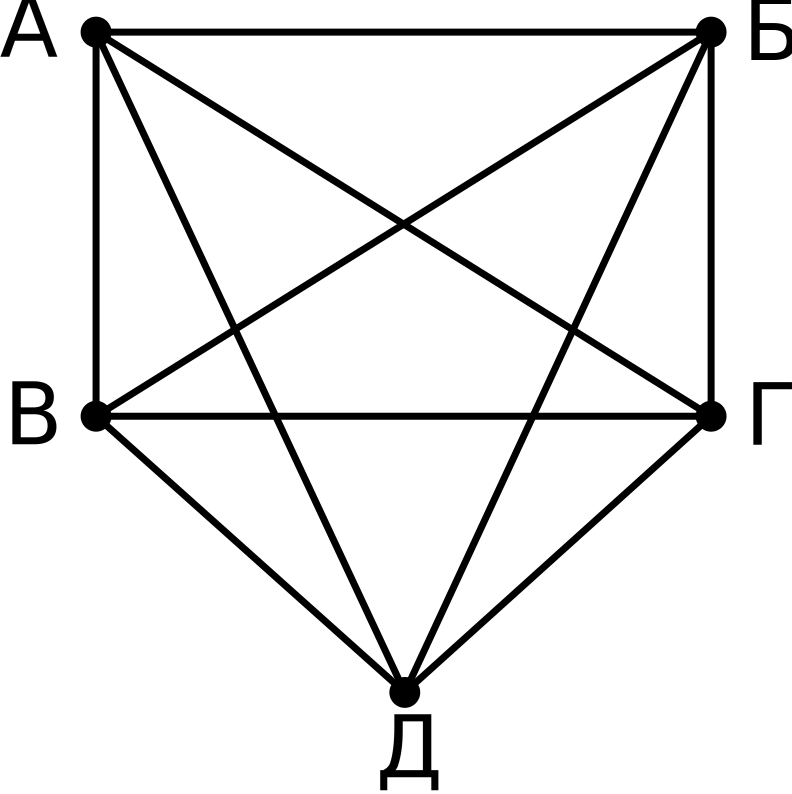
\includegraphics[width=0.4\textwidth]{images/graph-combinatorics.png}
        \caption{Решение с помощью графа}
    \end{figure}

    Решение для случая \(n\):
    \[
        (n - 1) + (n - 2) + \ldots + \ldots + 1 + 0 = \frac{n -1 + 0}{2} n = \frac{n(n - 1)}{2}.
    \]
\end{example}

\subsection{Правила суммы и произведения}

Если объект первого вида можно выбрать \(m\) способами, а объект второго вида -- \(n\) способами, то
\begin{itemize}
    \item один объект любого из этих видов можно выбрать \(m + n\) способами (правило суммы);
    \item пару объектов, один из которых первого вида, а другой -- второго вида, можно выбрать \(m \cdot n\) способами (правило произведения).
\end{itemize}

\begin{note*}
    Правила суммы и произведения справедливы для любого конечного числа видов объектов.
\end{note*}

\begin{example}
    В вазе лежит \(5\) яблок и \(3\) персика различных сортов. Сколькими способами можно выбрать один фрукт?

    По правилу суммы \(5 + 3 = 8\) вариантов.
\end{example}

\begin{example}
    Имеется \(2\) конверта: обычный и авиа, и \(3\) марки: прямоугольная, квадратная и треугольная. Сколькими способами можно выбрать конверт и марку, чтобы отправить письмо?

    По правилу произведения \(2 \cdot 3 = 6\) вариантов.
\end{example}

\begin{example}
    Сколько трехзначных чисел можно составить из \(1, 3, 5, 7\), используя в записи числа каждую из них не более одного раза?

    По правилу произведения \(4 \cdot 3 \cdot 2 = 24\) числа.
\end{example}

\begin{example}
    Сколько трехзначных чисел можно составить из \(1, 3, 5, 7\), используя в записи числа каждую из них любое число раз?

    По правилу произведения \(4 \cdot 4 \cdot 4 = 64\) числа.
\end{example}

\subsection{Схема выбора без возвращения}

\subsubsection{Перестановки}

Пусть имеется множество из \(n\) элементов. Каждая последовательность всех его элементов называется \textbf{перестановкой} из \(n\) элементов. Число всех перестановок из \(n\) элементов обозначается \(P_n\) и вычисляется по формуле:
\[
    P_n = n \cdot (n - 1) \cdot (n - 2) \cdot \ldots \cdot 1 = 1 \cdot 2 \cdot \ldots \cdot n = n!.
\]

\begin{example*}
    Имеется \(10\) различных книг. Сколько существует способов расставить их на одной книжной полке?

    Решение:
    \[
        n = 10
        \implies
        P_n = P_{10} = 10! = 3628800.
    \]
\end{example*}

\subsubsection{Размещения}

Пусть имеется множество из \(n\) элементов. \textbf{Упорядоченными подмножествами} этого множества называют различные последовательности, составленные из элементов подмножеств.

Каждое упорядоченное подмножество из \(k\) элементов множества из \(n\) элементов называется \textbf{размещением} из \(n\) элементов по \(k\) элементам. Число всех размещений из \(n\) элементов по \(k\) элементам обозначается \(A_n^k\) (читается <<\(A\) из \(n\) по \(k\)>>) и вычисляется по формуле:
\[
    A_n^k = n \cdot (n - 1) \cdot \ldots \cdot (n - k + 1) = \frac{n!}{(n - k)!}.
\]

\begin{example*}
    В турнире участвуют \(8\) спортсменов. Сколько можно сделать предсказаний относительно распределения первых трех мест?

    Решение:
    \[
        n = 8, k = 3
        \implies
        A_n^k = A_8^3 =
        \frac{8!}{(8 - 3)!} = 336.
    \]
\end{example*}

\begin{note*}
    Размещение \(A_n^n\) из \(n\) элементов по \(n\) элементам является перестановкой \(P_n\) из \(n\) элементов.
\end{note*}

\subsubsection{Сочетания}

Пусть имеется множество из \(n\) элементов. Каждое его подмножество из \(k\) элементов называется \textbf{сочетанием} из \(n\) элементов по \(k\) элементам. Таким образом, подмножества, отличающиеся друг от друга только порядком следования элементов, не считаются различными. Число всех сочетаний из \(n\) элементов по \(k\) элементам обозначается \(C_n^k\) (читается <<\(C\) из \(n\) по \(k\)>>) и вычисляется по формуле:
\[
    C_n^k = \frac{A_n^k}{k!} = \frac{n!}{k! (n - k)!}.
\]

\begin{example*}
    В группе \(25\) студентов. Надо выбрать трех человек, которые будут представлять группу на студенческой конференции. Сколькими способами можно осуществить этот выбор?

    Решение:
    \[
        n = 25, k = 3
        \implies
        C_n^k = C_{25}^3 = \frac{25!}{3! (25 - 3)!} = 2300.
    \]
\end{example*}

\subsection{Схема выбора с возвращением (с повторениями)}

\subsubsection{Перестановки с повторениями}

Пусть имеется мультимножество из \(n\) элементов \(k\) различных видов такое, что оно состоит из \(n_1\) элементов 1-го вида, \(n_2\) элементов 2-го вида, \ldots, \(n_k\) элементов \(k\)-го вида, причем \(n_1 + n_2 + \ldots + n_k = n\). Перестановки всех элементов такого мультимножества называются \textbf{перестановками с повторениями}.

\begin{theorem*}
    Число различных перестановок с повторениями равно
    \[
        P(n, n_1, \ldots, n_k) = \frac{n!}{n_1! \cdot \ldots \cdot n_k!}.
    \]
\end{theorem*}

\begin{example*}
    Определить, сколько различных слов можно составить из слова <<математика>>.

    В слове <<математика>> имеется 6 видов букв:
    \begin{multicols}{3}
        \begin{itemize}[label={}]
            \item букв <<м>> \(n_1 = 2\),
            \item букв <<е>> \(n_4 = 1\),
        \end{itemize}
        \begin{itemize}[label={}]
            \item букв <<а>> \(n_2 = 3\),
            \item букв <<и>> \(n_5 = 1\),
        \end{itemize}
        \begin{itemize}[label={}]
            \item букв <<т>> \(n_3 = 2\),
            \item букв <<к>> \(n_6 = 1\).
        \end{itemize}
    \end{multicols}
    Всего \(n = 2 + 3 + 2 + 1 + 1 + 1 = 10\) букв. Тогда из слова <<математика>> можно составить
    \[
        P(n, n_1, \ldots, n_6) = \frac{n!}{n_1! \cdot \ldots \cdot n_6!} = \frac{10!}{2! \cdot 3! \cdot 2! \cdot 1! \cdot 1! \cdot 1!} = 151200.
    \]
    различных слов.
\end{example*}

\subsubsection{Размещения с повторениями}

Пусть имеется множество из \(n\) элементов. Каждый кортеж длины \(k\), составленный из элементов данного \(n\)-элементного множества (элементы кортежа не обязательно должны быть различными), называется \textbf{размещением} из \(n\) элементов по \(k\) элементам \textbf{с повторениями}.

\begin{theorem*}
    Число всех размещений из \(n\) элементов по \(k\) элементам с повторениями равно:
    \[
        \bar{A}_n^k = \underbrace{n \cdot n \cdot \ldots \cdot n}_k = n^k.
    \]
\end{theorem*}

\begin{example*}
    Сколько пятизначных номеров можно составить из элементов множества \(\{1, 2, 3\}\)?

    Решение:
    \[
        n = 3, k = 5
        \implies
        \bar{A}_n^k = \bar{A}_3^5 = 3^5 = 243.
    \]
\end{example*}

\subsubsection{Сочетания с повторениями}

Пусть имеются элементы \(n\) различных видов. Из них составляется комбинация из \(k\) элементов такая, что порядок элементов в комбинации не важен, причем элементы одного вида могут повторяться. Такая комбинация называется \textbf{сочетанием с повторениями} из \(n\) элементов по \(k\) элементам.

\begin{theorem*}
    Число всех сочетаний с повторениями из \(n\) элементов по \(k\) элементам равно
    \[
        \bar{C}_n^k = C_{n + k - 1}^k.
    \]
\end{theorem*}

\begin{example*}
    В почтовом отделении продаются открытки пяти видов. Определить число способов покупки семи открыток.

    Решение:
    \[
        n = 5, k = 7
        \implies
        \bar{C}_n^k = \bar{C}_5^7 = C_{5 + 7 - 1}^7 = C_{11}^7 = 330.
    \]
\end{example*}

\subsection{Бином Ньютона}

Для произвольного положительного целого числа \(n\) справедлива следующая формула:
\[
    (a + b)^n =
    C_n^0 a^{n - 0} b^0 + C_n^1 a^{n - 1} b^1 + \ldots + C_n^n a^0 b^{n - 0} =
    \sum_{k = 0}^n C_n^k a^{n - k} b^k.
\]

Коэффициенты \(C_n^k\) называются \textbf{биномиальными коэффициентами} и вычисляются по формуле
\[
    C_n^k = \frac{n!}{k! (n - k)!}.
\]

\begin{example*}
    Определить разложение \((a + b)^n\) при \(n = 4\).

    Решение:
    \begin{gather*}
        (a + b)^4 =
        C_4^0 a^{4 - 0} b^0 + C_4^1 a^{4 - 1}b^1 + C_4^2 a^{4 - 2} b^2 + C_4^3 a^{4 - 3} b^3 + C_4^4 a^{4 - 4} b^4 = \\ =
        \frac{4!}{0! \cdot (4 - 0)!} a^4 + \frac{4!}{1! \cdot (4 - 1)!} a^3 b + \frac{4!}{2! \cdot (4 - 2)!} a^2 b^2 + \frac{4!}{3! \cdot (4 - 3)!} a b^3 + \\ + \frac{4!}{4! \cdot (4 - 4)!} b^4 =
        a^4 + 4 a^3 b + 6  a^2 b^2 + 4 a b^3 + b^4.
    \end{gather*}
\end{example*}

\subsection{Свойства биномиальных коэффициентов}

\begin{property}
    \[
        C_n^k = C_n^{n - k}.
    \]
    \begin{proof}
        \[
            C_n^{n - k} = \frac{n!}{(n - k)!(n - (n - k!))!} = \frac{n!}{(n - k)! k!} = \frac{n!}{k! (n - k)!} = C_n^k.
        \]
    \end{proof}
\end{property}

\begin{property}
    \[
        C_n^k = C_{n - 1}^k + C_{n - 1}^{k - 1}.
    \]
    \begin{proof}
        \begin{gather*}
            C_{n - 1}^k + C_{n - 1}^{k - 1} =
            \frac{(n - 1)!}{k! (n - 1 - k)!} + \frac{(n - 1)!}{(k - 1)! (n - 1 - k + 1)} = \\ =
            \frac{(n - 1)!}{(k - 1)! (n - k - 1)!} \Big( \frac{1}{k} + \frac{1}{n - k} \Big) =
            \frac{(n - 1)!}{(k - 1)! (n - k - 1)!} \cdot \frac{n - k + k}{k (n - k)} = \\ =
            \frac{(n - 1)! n}{(k - 1)! k (n - k - 1)! (n - k)} =
            \frac{n!}{k! (n - k)!} = C_n^k.
        \end{gather*}
    \end{proof}
\end{property}

\begin{property}
    \[
        C_n^i \cdot C_i^k = C_n^k \cdot C_{n - k}^{i - k}.
    \]
\end{property}

\begin{property}
    \[
        \sum_{k = 0}^n C_n^k = 2^n.
    \]
    \begin{proof}
        \[
            2^n = (1 + 1)^n = \sum_{k = 0}^n C_n^k \cdot 1^{n - k} \cdot 1^k = \sum_{k = 0}^n C_n^k.
        \]
    \end{proof}
\end{property}

\begin{property}
    \[
        \sum_{k = 0}^n (-1)^k C_n^k = 0.
    \]
\end{property}

\begin{property}
    \[
        \sum_{k = 0}^n k C_n^k = n 2^{n - 1}.
    \]
\end{property}

\begin{property}[тождество Коши]
    \[
        C_{m + n}^k = \sum_{i = 0}^k C_m^i C_n^{k - i}
    \]
\end{property}

\subsection{Треугольник Паскаля}

Рассмотрим следующий треугольник:

{
\renewcommand*{\arraystretch}{1.5}
\begin{longtable}{ccccccccc}
           &           &           &           & \(C_0^0\) &           &           &           &        \\
           &           &           & \(C_1^0\) &           & \(C_1^1\) &           &           &        \\
           &           & \(C_2^0\) &           & \(C_2^1\) &           & \(C_2^2\) &           &        \\
           & \(C_3^0\) &           & \(C_3^1\) &           & \(C_3^2\) &           & \(C_3^3\) &        \\
    \ldots &           & \ldots    &           & \ldots    &           & \ldots    &           & \ldots \\
\end{longtable}
}

Первая строка, состоящая из одного элемента, считается нулевой. Строка под номером \(n\) содержит биномиальные коэффициенты разложения \((a + b)^n\), то есть \(C_n^k\), где \(k\) пробегает значения от \(0\) до \(n\).

Элемент нулевой строки и боковые элементы треугольника равны единицам, а каждый внутренний элемент треугольника согласно свойству
\[
    C_n^k = C_{n - 1}^{k - 1} + C_{n - 1}^k
\]
равен сумме двух элементов, расположенных над ним. Таким образом, будем иметь:

{
\setlength{\tabcolsep}{3pt}
\begin{longtable}{ccccccccccccccccccccc}
           &       &        &       &        &        &        &        &        &         & \(1\)  &         &        &        &        &        &        &       &        &       &        \\
           &       &        &       &        &        &        &        &        & \(1\)   &        & \(1\)   &        &        &        &        &        &       &        &       &        \\
           &       &        &       &        &        &        &        & \(1\)  &         & \(2\)  &         & \(1\)  &        &        &        &        &       &        &       &        \\
           &       &        &       &        &        &        & \(1\)  &        & \(3\)   &        & \(3\)   &        & \(1\)  &        &        &        &       &        &       &        \\
           &       &        &       &        &        & \(1\)  &        & \(4\)  &         & \(6\)  &         & \(4\)  &        & \(1\)  &        &        &       &        &       &        \\
           &       &        &       &        & \(1\)  &        & \(5\)  &        & \(10\)  &        & \(10\)  &        & \(5\)  &        & \(1\)  &        &       &        &       &        \\
           &       &        &       & \(1\)  &        & \(6\)  &        & \(15\) &         & \(20\) &         & \(15\) &        & \(6\)  &        & \(1\)  &       &        &       &        \\
           &       &        & \(1\) &        & \(7\)  &        & \(21\) &        & \(35\)  &        & \(35\)  &        & \(21\) &        & \(7\)  &        & \(1\) &        &       &        \\
           &       & \(1\)  &       & \(8\)  &        & \(28\) &        & \(56\) &         & \(70\) &         & \(56\) &        & \(28\) &        & \(8\)  &       & \(1\)  &       &        \\
           & \(1\) &        & \(9\) &        & \(36\) &        & \(84\) &        & \(126\) &        & \(126\) &        & \(84\) &        & \(36\) &        & \(9\) &        & \(1\) &        \\
    \ldots &       & \ldots &       & \ldots &        & \ldots &        & \ldots &         & \ldots &         & \ldots &        & \ldots &        & \ldots &       & \ldots &       & \ldots \\
\end{longtable}
}

\begin{example}
    Используя треугольник Паскаля, найти \(C_5^2 + C_7^4 + C_9^6\).

    Решение:
    \[
        C_5^2 + C_7^4 + C_9^6 = 10 + 35 + 84 = 129.
    \]
\end{example}

\begin{example}
    Используя треугольник Паскаля, представить \((a + b)^7\) в виде многочлена:

    Решение:
    \[
        (a + b)^7 =
        a^7 + 7 a^6 b + 21 a^5 b^2 + 35 a^4 b^3 + 35 a^3 b^4 + 21 a^2 b^5 + 7 a b^6 + b^7.
    \]
\end{example}

\subsection{Полиномиальная формула}

Формула, обобщающая формулу бинома Ньютона, называется \textbf{полиномиальной}.

\begin{theorem*}
    Для любых натуральных чисел \(n\) и \(k\) и любых чисел \(a_1, \ldots, a_k\) справедлива формула
    \[
        (a_1 + \ldots + a_k)^n =
        \sum_{n_1 + \ldots + n_k = n} C(n, n_1, \ldots, n_k) \cdot a_1^{n_1} \cdot \ldots \cdot a_k^{n_k},
    \]
    где суммирование производится по всем решениям уравнения
    \[
        n_1 + n_2 + \ldots + n_k = n
    \]
    в неотрицательных целых числах.
\end{theorem*}

Коэффициенты данного разложения \(C(n, n_1, \ldots, n_k)\) называются \textbf{мультиномиальными коэффициентами} и вычисляются по формуле
\[
    C(n, n_1, \ldots, n_k) = \frac{n!}{n_1! \cdot \ldots \cdot n_k!}.
\]

Они совпадают с числом различных перестановок с повторениями:
\[
    P(n, n_1, \ldots, n_k) = \frac{n!}{n_1! \cdot \ldots \cdot n_k!}.
\]

\begin{example}
    Найти разложение степени \((a + b + c)^3\).

    Сначала определим число слагаемых в разложении:
    \[
        \bar{C}_3^3 = C_5^3 = \frac{5!}{3! \cdot 2!} = 10.
    \]
    \[
        (a + b + c)^3 = \sum_{n_1 + n_2 + n_3 = 3} C(3, n_1, n_2, n_3) a_1^{n_1} a_2^{n_2} a_3^{n_3},
    \]

    где
    \[
        C(3, n_1, n_2, n_3) = \frac{3!}{n_1! \cdot n_2! \cdot n_3!}.
    \]

    Возможно \(10\) решений уравнения \(n_1 + n_2 + n_3 = 3\) в целых числах:
    \begin{multicols}{2}
        \begin{enumerate}
            \item \(n_1 = 3\), \(n_2 = 0\), \(n_3 = 0\);
            \item \(n_1 = 2\), \(n_2 = 1\), \(n_3 = 0\);
            \item \(n_1 = 2\), \(n_2 = 0\), \(n_3 = 1\);
            \item \(n_1 = 1\), \(n_2 = 2\), \(n_3 = 0\);
            \item \(n_1 = 1\), \(n_2 = 1\), \(n_3 = 1\);
        \end{enumerate}
        \begin{enumerate}
            \setcounter{enumi}{5}
            \item \(n_1 = 1\), \(n_2 = 0\), \(n_3 = 2\);
            \item \(n_1 = 0\), \(n_2 = 3\), \(n_3 = 0\);
            \item \(n_1 = 0\), \(n_2 = 2\), \(n_3 = 1\);
            \item \(n_1 = 0\), \(n_2 = 1\), \(n_3 = 2\);
            \item \(n_1 = 0\), \(n_2 = 0\), \(n_3 = 3\).
        \end{enumerate}
    \end{multicols}

    \begin{gather*}
        (a + b + c)^3 =
        \frac{3!}{3! \cdot 0! \cdot 0!} a^3 b^0 c^0 + \frac{3!}{2! \cdot 1! \cdot 0!} a^2 b^1 c^0 + \frac{3!}{2! \cdot 0! \cdot 1!} a^2 b^0 c^1 + \\ + \frac{3!}{1! \cdot 2! \cdot 0!} a^1 b^2 c^0 + \frac{3!}{1! \cdot 0! \cdot 2!} a^1 b^0 c^2 + \frac{3!}{0! \cdot 2! \cdot 1!} a^0 b^2 c^1 + \frac{3!}{0! \cdot 1! \cdot 2!} a^0 b^1 c^2 + \\ + \frac{3!}{1! \cdot 1! \cdot 1!} a^1 b^1 c^1 + \frac{3!}{0! \cdot 3! \cdot 0!} a^0 b^3 c^0 + \frac{3!}{0! \cdot 0! \cdot 3!} a^0 b^0 c^3 = \\ =
        a^3 + 3 a^2 b + 3 a^2 c + 3 a b^2 + 3 a c^2 + 3 b^2 c + 3 b c^2 + 6 a b c + b^3 + c^3.
    \end{gather*}
\end{example}

\begin{example}
    В разложении многочлена \((1 + 2x^2 - 3x^4)^{10}\) найти коэффициент при \(x^8\).

    \begin{gather*}
        (1 + 2x^2 - 3x^4)^{10} =
        \sum_{n_1 + n_2 + n_3 = 10} \frac{10!}{n_1! \cdot n_2! \cdot n_3!} \cdot (1)^{n_1} \cdot (2x^2)^{n_2} \cdot (-3x^4)^{n_3} = \\ =
        \sum_{n_1 + n_2 + n_3 = 10} = \frac{10!}{n_1! \cdot n_2! \cdot n_3!} \cdot (2)^{n_2} \cdot (-3)^{n_3} \cdot x^{2n_2 + 4n_3}.
    \end{gather*}

    \[
        \begin{dcases}
            n_1 + n_2 + n_3 = 10 \\
            2n_2 + 4n_3 = 8.
        \end{dcases}
    \]

    \begin{enumerate}
        \item \(n_1 = 8\), \(n_2 = 0\), \(n_3 = 2\);
        \item \(n_1 = 7\), \(n_2 = 2\), \(n_3 = 1\);
        \item \(n_1 = 6\), \(n_2 = 4\), \(n_3 = 0\).
    \end{enumerate}

    Коэффициент при \(x^8\) вычисляется по формуле:
    \[
        \frac{10!}{n_1! \cdot n_2! \cdot n_3!} \cdot (2)^{n_2} \cdot (-3)^{n_3}.
    \]

    \begin{enumerate}
        \item \(n_1 = 8\), \(n_2 = 0\), \(n_3 = 2\):
              \[
                  \frac{10!}{8! \cdot 0! \cdot 2!} \cdot 2^0 \cdot (-3)^2 = 405;
              \]
        \item \(n_1 = 7\), \(n_2 = 2\), \(n_3 = 1\):
              \[
                  \frac{10!}{7! \cdot 2! \cdot 1!} \cdot 2^2 \cdot (-3)^1 = -4320;
              \]
        \item \(n_1 = 6\), \(n_2 = 4\), \(n_3 = 0\).
              \[
                  \frac{10!}{6! \cdot 4! \cdot 0!} \cdot 2^4 \cdot (-3)^0 = 3360.
              \]
    \end{enumerate}

    Таким образом, коэффициент при \(x^8\) будет равен:
    \[
        405 - 4320 + 3360 = -555.
    \]
\end{example}

\subsection{Схема упорядоченных разбиений}

Пусть имеется \(n\) различных шаров и \(k\) различных урн. Требуется разложить шары по урнам так, чтобы в \(i\)-й находилось \(m_i\) шаров, \(i = \overline{1, k}\), причем
\[
    m_1 + m_2 + \ldots + m_k = n.
\]
\[
    C(n, m_1, \ldots, m_k) = \frac{n!}{m_1! \cdot \ldots \cdot m_k!}.
\]

\begin{example}
    Известно, что принимая экзамен в группе из \(20\) человек, преподаватель поставил \(4\) <<пятерки>>, \(8\) <<четверок>>, \(5\) <<троек>> и \(3\) <<двойки>>. Сколько существует различных вариантов сдачи экзамена группой?

    Решение:
    \[
        C(20, 4, 8, 5, 3) = \frac{20!}{4! \cdot 8! \cdot 5! \cdot 3!} = 3491888400.
    \]
\end{example}

\subsection{Формула включений и исключений}

Формула, известная как \textbf{формула включений и исключений} позволяет вычислить мощность объединения множеств, если известны их мощности и мощности всех возможных пересечений.

\begin{theorem*}
    Пусть \(A_1, \ldots, A_n\) -- конечные множества. Тогда
    \begin{gather*}
        |A_1 \cup \ldots \cup A_n| =
        \sum_{1 \leq i_1 \leq n} |A_{i_1}| - \sum_{1 \leq i_1 < i_2 \leq n} |A_{i_1} \cap A_{i_2}| + \\ + \sum_{1 \leq i_1 < i_2 < i_3 \leq n} |A_{i_1} \cap A_{i_2} \cap A_{i_3}| - \ldots + (-1)^{n - 1} |A_1 \cap \ldots \cap A_n|.
    \end{gather*}
\end{theorem*}

\noindent Рассмотрим случай при \(n = 2\):
\[
    |A \cup B| = |A| + |B| - |A \cap B|.
\]

\noindent Рассмотрим случай при \(n = 3\):
\[
    |A \cup B \cup C| = |A| + |B| + |C| - |A \cap B|  - |A \cap B| - |B \cap C| + |A \cap B \cap C|.
\]

\noindent Рассмотрим случай при \(n = 4\):
\begin{gather*}
    |A \cup B \cup C \cup D| =
    |A| + |B| + |C| + |D| - |A \cap B| - |A \cap C| - |A \cap D| - \\ - |B \cap C| - |B \cap D| - |C \cap D| + |A \cap B \cap C| + |A \cap B \cap D| + \\ + |A \cap C \cap D| + |B \cap C \cap D| - |A \cap B \cap C \cap D|.
\end{gather*}

\begin{example}
    Сколько натуральных чисел в первой сотне, которые не делятся ни на \(2\), ни на \(5\), ни на \(7\)?
    \begin{gather*}
        A = \{ x \in \mathbb{N} \mid x \leq 100 \; \land \; x \divby 2 \},
        \qquad
        B = \{ x \in \mathbb{N} \mid x \leq 100 \; \land \; x \divby 5 \},
        \\
        C = \{ x \in \mathbb{N} \mid x \leq 100 \; \land \; x \divby 7 \}.
    \end{gather*}
    \[
        |A \cup B \cup C| = |A| + |B| + |C| + |A \cap B| - |A \cap C| - |B \cap C| + |A \cap B \cap C|.
    \]
    \[
        \overline{|A \cup B \cup C|} = |U| - |A \cup B \cup C|.
    \]
    \begin{gather*}
        |A| = \Bigg[ \frac{100}{2} \Bigg] = 50,
        \quad
        |B| = \Bigg[ \frac{100}{5} \Bigg] = 20,
        \quad
        |C| = \Bigg[ \frac{100}{7} \Bigg] = 14,
        \\
        |A \cap B| = \Bigg[ \frac{100}{\nok(2, 5)} \Bigg] = \Bigg[ \frac{100}{2 \cdot 5} \Bigg] = 10, \\
        |A \cap C| = \Bigg[ \frac{100}{\nok(2, 7)} \Bigg] = \Bigg[ \frac{100}{2 \cdot 7} \Bigg] = 7, \\
        |B \cap C| = \Bigg[ \frac{100}{\nok(5, 7)} \Bigg] = \Bigg[ \frac{100}{5 \cdot 7} \Bigg] = 2, \\
        |A \cap B \cap C| = \Bigg[ \frac{100}{\nok(2, 5, 7)} \Bigg] = \Bigg[ \frac{100}{2 \cdot 5 \cdot 7} \Bigg] = 1.
    \end{gather*}
    \[
        |A \cup B \cup C| = 50 + 20 + 14 - 10 - 7 - 2 + 1 = 66.
    \]
    \[
        \overline{|A \cup B \cup C|} = 100 - 66 = 34.
    \]

    \textbf{Ответ}: 34.
\end{example}

\begin{example}
    Человек хочет послать своему другу \(8\) различных фотографий. Сколькими способами он может это сделать, использовав \(5\) различных конвертов, если ни один конверт не должен быть пустым?

    Решение:
    \[
        5^8 - C_5^1 \cdot 4^8 + C_5^2 \cdot 3^8 - C_5^3 \cdot 2^8 + C_5^4 \cdot 1^8 = 126000.
    \]
\end{example}

\begin{example}
    Сколькими способами можно положить \(n\) различных предметов в \(m\) различных ящиков так, чтобы в каждом ящике лежал хотя бы один предмет?

    Решение:
    \[
        m^n - C_m^1 (m - 1)^n + C_m^2 (m - 2)^n - \ldots + (-1)^{m - 1} C_m^{m - 1} \cdot 1^n.
    \]
\end{example}

\begin{example}
    Сколькими способами можно положить \(n\) различных предметов в \(m\) \textbf{неразличимых} ящиков так, чтобы в каждом ящике лежат хотя бы один предмет?

    Решение:
    \[
        \frac{1}{m!} \Big( m^n - C_m^1 (m - 1)^n + C_m^2 (m - 2)^n - \ldots + (-1)^{m - 1} C_m^{m - 1} \cdot 1^n \Big).
    \]

    Полученная формула также называется \textbf{числом Стирлинга второго рода}.
\end{example}

\subsection{Задача о беспорядках}

\textbf{Беспорядком} называют перестановку \(n\) различных элементов, в которой ни один предмет не останется на своем первоначальном месте. Количество всех беспорядков обозначается \(D(n)\) и вычисляется по формуле:
\[
    D(n) = n! - C_n^1 (n - 1)! + C_n^2 (n - 2)! - \ldots + (-1)^n C_n^n (n - n)!.
\]

Учитывая, что
\[
    C_n^k \cdot (n - k)! = \frac{n!}{k!}
\]
формулу можно записать следующим образом:
\[
    D(n) =
    n! - \frac{n!}{1!} + \frac{n!}{2!} - \ldots + (-1)^n \frac{n!}{n!} =
    n! \Big( 1 - \frac{1}{1!} + \frac{1}{2!} - \ldots + (-1)^n \frac{1}{n!} \Big).
\]

Количество перестановок \(n\) различных предметов, при которых \(k\) предметов стоят на своих первоначальных местах, выражается числом
\[
    D(n, k) = C_n^k \cdot D(n - k).
\]

\subsection{Разбиения}

Пусть \(\{B_1, \ldots, B_k\}\) -- \textbf{разбиение} множества \(X\) из \(n\) элементов на \(k\) подмножеств:
\[
    B_i \subset X,
    \quad
    \bigcup_{i - 1}^k B_i = X,
    \quad
    B_i \neq \varnothing,
    \quad
    B_i \cap B_j = \varnothing \; \text{при} \; i \neq j.
\]
Подмножества \(B_i\) называются \textbf{блоками разбиения}.

\subsection{Число Стирлинга второго рода}

Число разбиений множества из \(n\) элементов на \(k\) непустых подмножеств (блоков) называется \textbf{числом Стирлинга второго рода} и обозначается \(S(n, k)\) или \(\displaystyle \begin{Bmatrix} n \\ k \end{Bmatrix} \) (читается <<\(k\) подмножеств из \(n\)>>). По определению полагают:
\begin{gather*}
    S(n, n) = 1,
    \quad
    S(n, 0) = 0 \; \text{при} \; n > 0,
    \\
    S(0, 0) = 1,
    \quad
    S(n, k) = 0 \; \text{при} \; k > n.
\end{gather*}

\textbf{Рекуррентная формула}:
\[
    S(n, k) = S(n - 1, k -1) + k \cdot S(n - 1, k) \; \text{для} \; 0 < k < n.
\]

\textbf{Явная формула}:
\[
    S(n, k) = \frac{1}{k!} \sum_{i = 0}^k (-1)^{k + i} C_k^i \cdot i^n.
\]

Число размещений \(n\) предметов по \(k\) ящикам так, чтобы все ящики были заняты, вычисляется по формуле
\[
    k! \cdot S(n, k).
\]

\begin{example}
    Найти число разбиений четырехэлементного множества на две части. Пусть таким четырехэлементным множеством будет множество \(\{1, 2, 3, 4\}\). Тогда получим следующие разбиения:
    \begin{gather*}
        \{1, 2, 3\} \cup \{4\},
        \quad
        \{1, 2, 4\} \cup \{3\},
        \quad
        \{1, 3, 4\} \cup \{2\},
        \quad
        \{2, 3, 4\} \cup \{1\}, \\
        \quad
        \{1, 2\} \cup \{3, 4\},
        \quad
        \{1, 3\} \cup \{2, 4\},
        \quad
        \{1, 4\} \cup \{2, 3\}.
    \end{gather*}

    Итого получаем, что \(S(4, 2) = 7\). Получим тот же результат с помощью формулы:
    \[
        S(4, 2) =
        \frac{1}{2!} \Big( (-1)^2 C_2^0 0^4 + (-1)^3 C_2^1 1^4 + (-1)^4 C_2^2 2^4 \Big) =
        \frac{14}{2} = 7.
    \]
\end{example}

\begin{example}
    Найти число разбиений пятиэлементного множества на три части.

    Решение:
    \begin{gather*}
        S(5, 3) = \frac{1}{3!} \Big( (-1)^3 C_3^0 0^5 + (-1)^4 C_3^1 1^5 + (-1)^5 C_3^2 2^5 + (-1)^6 C_3^3 3^5 \Big) = \\
        = \frac{150}{6} = 25.
    \end{gather*}
\end{example}

\subsection{Число Белла}

Число всех разбиений множества из \(n\) элементов называется \textbf{числом Белла} и обозначается \(B(n)\):
\[
    B(n) = \sum_{k = 1}^n S(n, k),
    \qquad
    B(0) = 1.
\]

\begin{theorem*}
    Числа Белла удовлетворяют следующему рекуррентному соотношению:
    \[
        B(n + 1) = \sum_{k = 0}^n C_n^k B(k).
    \]
\end{theorem*}

\begin{example}
    Найти число всех возможных разбиений трехэлементного множества.

    Решение c помощью числа Белла:
    \begin{gather*}
        B(3) =
        \sum_{k = 1}^3 S(3, k) =
        S(3, 1) + S(3, 2) + S(3, 3) = \\ =
        1 + \frac{1}{2!} \Big( (-1)^2 C_2^0 0^3 + (-1)^3 C_2^1 1^3 + (-1)^4 C_2^2 2^3 \Big) + 1 =
        1 + \frac{6}{2} + 1 = 5.
    \end{gather*}

    Это легко проверить на примере множества \(\{a, b, c\}\):
    \begin{gather*}
        \{\{a\}, \{b\}, \{c\}\},
        \quad
        \{\{a, b\}, \{c\}\},
        \quad
        \{\{a, c\}, \{b\}\}, \\
        \quad
        \{\{a\}, \{b, c\}\},
        \quad
        \{\{a, b, c\}\}.
    \end{gather*}
\end{example}

\begin{example}
    Найти \(B(4)\), используя рекуррентное соотношение.

    Решение:
    \begin{gather*}
        B(4) =
        \sum_{k = 0}^3 C_3^k B(k) =
        C_3^0 B(0) + C_3^1 B(1) + C_3^2 B(2) + C_3^3 B(3) = \\ =
        1 \cdot 1 + 3 \cdot 1 + 3 \cdot 2 + 1 \cdot 5 =
        15.
    \end{gather*}
\end{example}

\subsection{Треугольник Белла}

\noindent Принцип построения треугольника Белла:
\begin{itemize}
    \item первая строка содержит \(1\);
    \item каждая следующая строка начинается числом, стоящим в конце предыдущей строки;
    \item каждое следующее число в строке равно сумме чисел, стоящих слева и сверху от него;
    \item числа Белла образуют последние числа в строках.
\end{itemize}

{
\renewcommand*{\arraystretch}{1.5}
\setlength{\tabcolsep}{1pt}
\begin{longtable}{ccccccccccccccccc}
               &         &            &          &            &          &            &          & \(1\)      &          &            &          &            &          &            &          &            \\
               &         &            &          &            &          &            & \(1\)    &            & \(2\)    &            &          &            &          &            &          &            \\
               &         &            &          &            &          & \(2\)      &          & \(3\)      &          & \(5\)      &          &            &          &            &          &            \\
               &         &            &          &            & \(5\)    &            & \(7\)    &            & \(10\)   &            & \(15\)   &            &          &            &          &            \\
               &         &            &          & \(15\)     &          & \(20\)     &          & \(27\)     &          & \(37\)     &          & \(52\)     &          &            &          &            \\
               &         &            & \(52\)   &            & \(67\)   &            & \(87\)   &            & \(114\)  &            & \(151\)  &            & \(203\)  &            &          &            \\
               &         & \(203\)    &          & \(255\)    &          & \(322\)    &          & \(409\)    &          & \(523\)    &          & \(674\)    &          & \(877\)    &          &            \\
               & \(877\) &            & \(1080\) &            & \(1335\) &            & \(1657\) &            & \(2066\) &            & \(2589\) &            & \(3263\) &            & \(4140\) &            \\
    \(\ldots\) &         & \(\ldots\) &          & \(\ldots\) &          & \(\ldots\) &          & \(\ldots\) &          & \(\ldots\) &          & \(\ldots\) &          & \(\ldots\) &          & \(\ldots\) \\
\end{longtable}
}

{
\renewcommand*{\arraystretch}{1.5}
\setlength{\tabcolsep}{10pt}
\begin{longtable}{|c|c|c|c|c|c|c|c|c|c|}
    \hline
    \(n\)    & \(0\) & \(1\) & \(2\) & \(3\) & \(4\)  & \(5\)  & \(6\)   & \(7\)   & \(8\)    \\
    \hline
    \(B(n)\) & \(1\) & \(1\) & \(2\) & \(5\) & \(15\) & \(52\) & \(203\) & \(877\) & \(4140\) \\
    \hline
\end{longtable}
}

\subsection{Числа Фибоначчи}

Числа Фибоначчи \(F(n)\) определяются следующим образом:
\[
    F(0) = 1,
    \quad
    F(1) = 1,
    \quad
    \forall n \; \geq 0 \; F(n + 2) = F(n + 1) + F(n).
\]

Последовательность Фибоначчи имеет вид:
\[
    1, 1, 2, 3, 5, 8, 13, 21, 34, 55, 89, 144, 233, \ldots.
\]

\(F(n + 2) - F(n + 1) - F(n) = 0\) представляет собой линейное однородное разностное уравнение второго порядка, его характеристическое уравнение имеет вид:
\[
    \lambda^2 - \lambda - 1 = 0
    \implies
    \lambda_{1, 2} = \frac{1 \pm \sqrt{5}}{2}.
\]

Положительный корень этого уравнения обозначается греческой буквой \(\Phi\) (фи):
\[
    \Phi = \frac{1 + \sqrt{5}}{2} \approx 1.618
\]
и называется <<Золотым сечением>>.

\textbf{Золотое сечение} -- это такое пропорциональное деление отрезка на неравные части, при котором весь отрезок так относится к большей части, как сама большая часть относится к меньшей (отношение меньшей части к большей равно отношению большей части к длине всего отрезка)
\[
    \lim_{n \to \infty} \frac{F(n + 1)}{F(n)} = \Phi.
\]

Формула для вычисления чисел Фибоначчи имеет вид:
\[
    F(n) = \frac{1}{\sqrt{5}} \Bigg( \bigg(\frac{1 + \sqrt{5}}{2} \bigg)^{n + 1} - \bigg( \frac{1 - \sqrt{5}}{2} \bigg)^{n + 1} \Bigg).
\]

\subsection{Числа Каталана}

Числа Каталана используются при решении различных комбинаторных задач, обозначаются \(C(n)\) и определяются следующим рекуррентным соотношением:
\[
    C(0) = 1,
    \qquad
    C(n) = \sum_{k = 0}^{n - 1} C(k) \cdot C(n - k - 1).
\]

Числа Каталана выражаются через биномиальные коэффициенты:
\[
    C(n) = \frac{C_{2n}^n}{n + 1} = \frac{1}{n + 1} C_{2n}^n
\]

Числа Каталана встречаются в большом количестве задач комбинаторики. Так, например, \(n\)-е число Каталана -- это:
\begin{itemize}
    \item количество корректных скобочных последовательностей, состоящих из \(n\) открывающих и \(n\) закрывающих скобок;
    \item количество корневых бинарных деревьев с \(n + 1\) листьями (вершины не пронумерованы);
    \item количество триангуляций выпуклого \(n + 2\)-угольника;
    \item количество способов соединить \(2n\) точек на окружности \(n\) непересекающимся хордами.
\end{itemize}

\end{document}
